\chapter{Advanced Technologies in Multimedia}


\section{Multimedia Operating System}
\subsection{Introduction}

The operating system is the shield of the computer hardware against all software components. It provides a comfortable environment for the execution of programs, and it ensures effective utilization of the computer hardware. The operating system offers various services related to the essential resources of a computer: CPU, main memory, storage and all input and output devices.

For the processing of audio and video, multimedia application demands that humans perceive these media in a natural, error-free way. These continuous media data originate at sources like microphones, cameras and files. From these sources, the data
are transferred to destinations like loudspeakers, video windows and files located at the same computer or at a remote station. On the way from source to sink, the digital data are processed by at least some type of move, copy or transmit operation. In this data
manipulation process there are always many resources which are under the control of the operating system. The integration of discrete and continuous multimedia data demands additional services from many operating system components.


\subsection{Resource Management}
%\begin{multicols}{2}
	Multimedia systems with their integrated audio and video processes often reach their capacity limits despite the usage of data compression and utilization of the newest computing and communication technologies. Current multimedia systems require therefore their own resource management; here the availability of resource reservation may provide an advantage for quality provision in these systems. 
	
	The actual requirements depend on the \textit{type of media} and the \textit{nature of the applications} supported. 
	
	In integrated distributed multimedia system, several applications compete for system resources. This shortage of resources requires careful allocation. The system management must employ adequate scheduling algorithms to serve the requirements of the applications. Thereby, the resource is first allocated and then
	managed
	
	Resource management in distributed multimedia systems covers several computers and the involved communication networks. It allocates all resources involved in the data transfer process between sources and sinks
	
	Applied to operating systems, resource management covers the CPU (including process management), memory management, the file system and device management
%\end{multicols}

\subsubsection{Resources}
A resource is a system entity required by tasks for manipulating data. Each resource has a set of distinguished characteristics, and they can be classified as follows:

\begin{itemize}
	\item A resource can be \textit{active} or \textit{passive}:
		\begin{itemize}
			\item An \textit{active resource} is the CPU or a network adapter for protocol processing; it provides a service.
			
			\item A \textit{passive resourc}e is the main memory, communication bandwidth or a file system; it denotes some system capability required by active resources.
		\end{itemize}
	 
	\item A resource can be either used \textit{exclusively} one process at a time or
	\textit{shared} between various processes
		\begin{itemize}
			\item Active resources are often exclusive
			\item passive resources can usually be shared among processes
		\end{itemize}
	
	 \item A resource that exists only once in the system is known as a \textit{single},
	 otherwise it is a \textit{multiple} resource.
\end{itemize}

\subsubsection{Requirements}
The requirements of multimedia applications and data streams must be served by the single components of a multimedia system. The transmission and processing requirements of local and distributed multimedia applications can be specified according to the following characteristics:

\begin{itemize}
	\item \textit{Throughput} can be determined from the needed data rate and the data unit size, transmitted over a connection.
	\item \textit{Delay} needs to be distinguished between the local and the global (end-to-end) delay:
		\begin{itemize}
			\item \textit{Local delay} is the maximum time span for the completion of a certain task at this resource.
			
			\item \textit{End-to-end delay} is the total delay for a data unit to be transmitted from the source to its destination.
		\end{itemize}
	
	\item \textit{Jitter} (or delay jitter) determines the maximum allowed variance in the arrival of data at the destination.
	
	\item \textit{Reliability} maps to the error handling algorithms. The reliability defines error detection and correction mechanisms used for the transmission and processing of multimedia tasks.
\end{itemize}

In accordance with communication systems, these requirements are also known as \textit{Quality of Service parameters (QoS)}.

\subsubsection{Allocation Scheme}
Reservation of resources can be made either in a pessimistic or optimistic way:

\begin{itemize}
	\item The \textit{pessimistic approach} avoids resource conflicts by making reservations for the worst case, i.\ e.\ resource bandwidth for the longest processing time and the highest rate which might ever be needed by a task is reserved. Resource conflicts are therefore avoided.
	
	\item With the \textit{optimistic approach}, resources are reserved according to an	average workload only. This means that the CPU is only reserved for the average processing time.
\end{itemize}

The optimistic approach is considered to be an extension of the pessimistic approach. It requires that additional mechanisms to detect and solve resource conflicts be implemented.

\subsubsection{Continuous Media Resource Model}
To present more precisely QoS parameters and the multimedia stream characteristics at the system level, often a continuous media model is considered.

Continuous media model is frequently adopted to define QoS parameters and hence, the characteristics of the data stream. It is based on the model of \textit{Linear Bounded Arrival Processes (LBAP)}. In this model a distributed system is decomposed into a chain of resources traversed by the messages on their end-to-end path.
		
LBAP model is a message arrival process at a resource defined by three parameters: 
\begin{multicols}{2}
	\begin{enumerate}
		\item \textit{Maximum message size} $ M $, measured in bytes per message ($ bytes/ Msg $)
		\item \textit{Maximum message rate} $ R $, measured in messages per second ($ Msg/s $), and 
		\item \textit{Maximum burstiness} $ B $ measured in messages ($ Msg $).
	\end{enumerate}
\end{multicols}


\paragraph*{Example}
The LBAP model is discussed in terms of a specific example: two workstations are interconnected by a LAN. A CD player is attached to one workstation. Single channel audio data are transferred from the CD player to this workstation over the network to the other computer. The audio signal is sampled with the frequency of $ 44.1 kHz $. Each sample is coded with $ 16 bits $. This results in a data rate of:
\begin{flalign*}
R_{byte} = 44,100Hz \times \frac{16bits}{8bits/byte} = 88,200 bytes/s
\end{flalign*}

The samples on a CD are assembled into frames. These frames are the audio messages to be transmitted. $ 75 $ of these audio messages are transmitted per	second. Therefore, we encounter a maximum message size of:	
\begin{flalign*}
	M= \frac{88,200 byte/s}{75Msg/s} = 1,176byte/Msg
\end{flalign*}

Up to $ 12,000 bytes $ are assembled into one packet and transmitted over LAN. In a packet of $ 12,000 bytes $ transmitted over the LAN, we will never encounter more messages than:
\begin{flalign*}
	\frac{12,000byte}{1,176byte/Msg} \geq 10 Msg = B
\end{flalign*}
It obviously follows that:
\begin{multicols}{3}
	\begin{itemize}
		\item $M= 1176 bytes/Msg$
		\item $R= 75 Msg/s$
		\item $B=10 Msg$
	\end{itemize}
\end{multicols}


\subsubsection*{Burst}
In the following calculation we assume that because of lower adjacent data rate, a burst never exceeds the maximum data rate. Hence, bursts do not succeed one another. During the time interval of length $ t $, the maximum number of messages arriving at a resource must not exceed:
\[\bar{M} = B + R \times t\]

For example, if we assume $ t = 1 s $, then
\[\bar{M}= 10 Msg + 75 Msg/ s  \times 1s = 85 Msg\]

The introduction of burstiness B allows for short time violations of the rate constraint.

\subsubsection*{Maximum Average Data Rate}
The maximum average data rate of the LBAP can be calculated as follows:
\[R=M \times R\]
For example:
\[R = 1,176 byte/Msg \times 75 Msg/s = 88,200 byte/s\]

\subsection{Process Management}
Process management deals with the resource \textit{main processor}. The capacity of this resource is specified as processor capacity. The process manager maps single processes onto resources according to a specified scheduling policy such that all processes meet their requirements. In most systems, a process under control of the process manager can adopt one of the following states:

\begin{multicols}{2}
	\begin{itemize}
		\item In the \textbf{initial state}, no process is assigned to the program. The process is in the idle state.
		\item If a process is waiting for an event, i.\ e.\ , the process lacks one of the necessary resources for processing. It is in the \textbf{blocked state}.
		\item If all necessary resources are assigned to the process, it is ready to run. The process only needs the processor for the execution of the program. The process is in the \textbf{ready state}.
		\item A process is running as long as the system processor is assigned to it. In this case, the process is in \textbf{running state}.
	\end{itemize}
\end{multicols}

 
The process manager is the \textit{scheduler}. This entity transfers a process into the ready-to-run state by assigning it a position in the respective queue of the dispatcher, which is the essential part of the operating system kernel. The dispatcher manages the context
switch and hence the transition from the ready-to-run to the run state. In most operating systems, the next process to run is chosen according to a priority policy. Between processes with the same priority, the one with the longest ready time is chosen.
	

\subsubsection{Real-time Processing Requirement}
Continuous media data processing must occur in exactly predetermined-usually periodic-intervals. Operations on these data recur over and over and must be completed at certain deadlines. The real-time process manager determines a schedule for the CPU resource CPU that allows it to make reservations and to give processing guarantees. The problem is to find a feasible scheduler which schedules all time-critical continuous media tasks in a way that each of them can meet its deadlines. This must be guaranteed for all tasks in every period for the whole run-time of the system. In a multimedia system, continuous and discrete media data are processed concurrently.

For scheduling of multimedia tasks, two conflicting goals must be considered:

\begin{multicols}{2}
\begin{itemize}
	\item An uncritical process should not suffer from starvation because time-critical	processes are executed. Multimedia applications rely as much on text and graphics as on audio and video.
		
	\item On the other hand, a time-critical process must never be subject to priority inversion.
	\end{itemize}
\end{multicols}


%Apart from the overhead caused by the schedulability test and the connection establishment, the costs for the scheduling of every message must be minimized. They are more
%critical because they occur periodically with every message during the processing of
%real-time tasks. The overhead generated by the scheduling and operating system is part
%of the processing time and therefore must be added to the processing time of the realtime tasks. Thus, it is favorable to keep them low. It is particularly difficult to observe
%the timing behavior of the operating system and its influence on the scheduling and the
%processing of time-critical data. It can lead to time garbling of application programs.
%Therefore, operating systems in real-time systems cannot be viewed as detached from
%the application programs and vice versa.

Realtime requirements of multimedia processes can be partitioned into two groups: 
\begin{multicols}{2}
	\begin{enumerate}
		\item hard-realtime requirements
		\item soft-realtime requirements
	\end{enumerate}
\end{multicols}

\textit{Hard-realtime} requirements mean that each deadline of a multimedia process must be guaranteed by the process management.

Soft-realtime requirements mean that most of the deadlines of a multimedia process are guaranteed by the process management, but some deadlines can be violated over the duration of the task without any catastrophic consequences.

\subsubsection*{Traditional Real-time Scheduling}
The problem of realtime processing is widely known in computer science. Some realtime scheduling methods are employed in operations research. They differ from computer science realtime scheduling because they operate in a static environment, where no adaptation to changes of the workload is necessary.

The goal of traditional scheduling on time-sharing computers is optimal throughput, optimal resource utilization and fair queuing. In contrast, the main goal of realtime tasks is to provide a schedule that allows all, respectively, as many time-critical processes as possible, to be processed in time, according to their deadline. 

There are several attempts to solve real-time scheduling problems. Many of them are just variations of basic algorithms. To find the best solutions for multimedia systems, two basic algorithms are analyzed:

\begin{multicols}{2}
	 \begin{enumerate}
		\item \textit{Earliest Deadline First} Algorithm
		\item \textit{Rate Monotonic Scheduling}
	\end{enumerate}
\end{multicols}


\subsubsection{Real-time Scheduling}
All scheduling algorithms to be introduced are based on the following system model for the scheduling of real-time tasks. Their essential components are the resources, tasks and scheduling goals.

A \textit{task} is a schedulable entity of the system, and it corresponds to the notion of a thread in the previous description. In a hard real-time system, a task is characterized by its timing constraints, as well as by its resource requirements. 

The time constraints of the periodic task $ T $ are characterized by the following parameters  ($ s $, $ e $, $ d $, $ p $):


%$\Theta$
\begin{multicols}{2}
	\begin{itemize}
		\item $ s $: Starting point
		\item $ e $: Processing time of $ T $
		\item $ d $: Deadline of $ T $
		\item $ p $: Period of $ T $
		\item $ r $: Rate of $ T(r=\frac{1}{p}) $
	\end{itemize}
\end{multicols}


%%%%%%%%%%%%%%%%%%%%%%%%%%%%%%%%%%%%%%%%%
%										%
%				FIGURE				   	%
%										%
%%%%%%%%%%%%%%%%%%%%%%%%%%%%%%%%%%%%%%%%%
\begin{figure}[ht!]
	\centering
	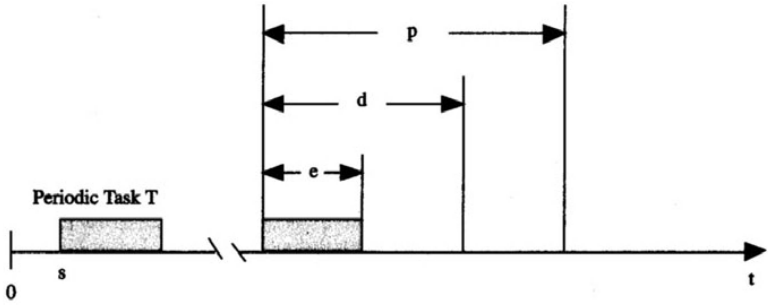
\includegraphics[width=0.8\textwidth]{periodic-tasks}
	\caption{Characterization of periodic tasks.}\label{fig:periodic-tasks}
\end{figure}
%--------------------------Figure end -------------------

\begin{multicols}{2}
	\begin{itemize}
		\item Whereby $0 \leq e \leq d \leq p $ (see Figure {\ref{fig:periodic-tasks}}). The starting point $ s $ is the first time when the periodic task requires processing.
		\item Afterwards, it requires processing in every period with a processing time of $ e $.
		\item At $ s + (k - 1) p $, the task $ T $ is ready for k-processing.
		\item The processing of $ T $ in period $ k $ must be finished at $ s + (k - 1) p + d  $.
		\item For continuous media tasks, it is assumed that the deadline of the period $ (k - 1) $ is the ready time of period $ k $.
		\item This is known as the congestion avoiding deadlines: the deadline for each message $ (d) $
		coincides with the period of the respective periodic task $ (p) $.
	\end{itemize}
\end{multicols}


Tasks can be \textit{preemptive} or \textit{non-preemptive}:
\begin{multicols}{2}
	\begin{itemize}
		\item A \textit{preemptive} task can be interrupted by the request of any task with a higher priority. Processing is continued in the same state later on. 
		\item A \textit{non-preemptive} task cannot be interrupted until it voluntarily yields the processor. Any high-priority task must wait until the low-priority task is finished. The high-priority task is then subject to priority inversion.
	\end{itemize}
\end{multicols}

 
A major performance metric for a real-time scheduling algorithm is the guarantee ratio. The guarantee ratio is the total number of guaranteed tasks versus the number of tasks which could be processed.

Another performance metric is the processor utilization. This is the amount of processing time used by guaranteed tasks versus the total amount of processing time:

\[
U={\sum_{i=1}^{n}} \frac{e_i}{p_i}
\]
	
\subsubsection[Earliest Deadline First Algorithm]{Earliest Deadline First (EDF) Algorithm}
\begin{multicols}{2}
	\begin{itemize}
		\item One of the best-known algorithms for real-time processing. 
		\item At every new ready state, the scheduler selects the task with the earliest deadline among the tasks. 
		\item The requested resource is assigned to the selected task. 
		\item At any arrival of a new task, EDF must be computed immediately leading to a new order.
		\item The new task is processed immediately if its deadline is earlier than that of the interrupted task. 
		\item The processing of the interrupted task is continued according to the EDF algorithm later on.
	\end{itemize}
\end{multicols}


EDF is an optimal, dynamic algorithm, i.\ e.\, it produces a valid schedule whenever one exists. With n tasks which have arbitrary ready-times and deadlines, the complexity is $ \Theta ( n^2)$ [ \textnp{याे uppercase Theta \(\Theta\) हो, lowercase Theta \(\theta\) होइन। }].

For scheduling continuous media data on a single processor machine with priority scheduling, process priorities are likely to be rearranged quite often. A priority is assigned to each task ready for processing according to its deadline. If the
computed priority of a new process is not available, the priorities of other processes must be rearranged until the required priority is free. In the worst case, the priorities of all processes must be rearranged.

\subsubsection{Rate Monotonic Algorithm}
The rate monotonic scheduling principle was introduced by Liu and Layland in 1973. It is an optimal, static, priority-driven algorithm for preemptive, periodic jobs. Optimal in this context means that there is no other static algorithm that is able to schedule a task set which cannot be scheduled by the rate monotonic algorithm. A process is scheduled by a static algorithm at the beginning of the processing. Subsequently, each task is processed with the priority calculated at the beginning. No further scheduling is required. The following five assumptions are necessary prerequisites to apply the
rate monotonic algorithm:

\begin{multicols}{2}
	\begin{enumerate}
		\item The requests for all tasks with deadlines are periodic, i.\ e.\ , have constant intervals between consecutive requests.
		\item The processing of a single task must be finished before the next task of the same	data stream becomes ready for execution. 
		Deadlines consist of runability constraints only, i.\ e.\ , each task must be completed before the next request occurs.
		\item All tasks are independent. 
		\item This means that the requests for a certain task do not depend on the initiation or completion of requests for any other task.
		\item Run-time for each request of a task is constant. 
		\item Run-time denotes the maximum time which is required by a processor to execute the task without interruption.
		
		\item Any non-periodic task in the system has no required deadline. 
		\item Typically, they initiate periodic tasks or are tasks for failure recovery. 
		\item They usually displace	periodic tasks.
	\end{enumerate}
\end{multicols}

The rate monotonic algorithm is a simple method to schedule time-critical, periodic tasks on the respective resource. A task will always meet its deadline, if this can be proven to be true for the longest response time. The response time is the time span between the request and the end of processing the task. This time span is maximal when all processes with a higher priority request to be processed at the same time. This case is known as the critical instant (see Figure \ref{fig:critical-instants}). In this figure, the priority of $ a $ is, according to the rate monotonic algorithm, higher than $ b $, and $ b $ is higher than $ c $. The critical time zone is the time interval between the critical instant and the completion of a task

%%%%%%%%%%%%%%%%%%%%%%%%%%%%%%%%%%%%%%%%%
%										%
%				FIGURE				   	%
%										%
%%%%%%%%%%%%%%%%%%%%%%%%%%%%%%%%%%%%%%%%%
\begin{figure}[pht]
	\centering
	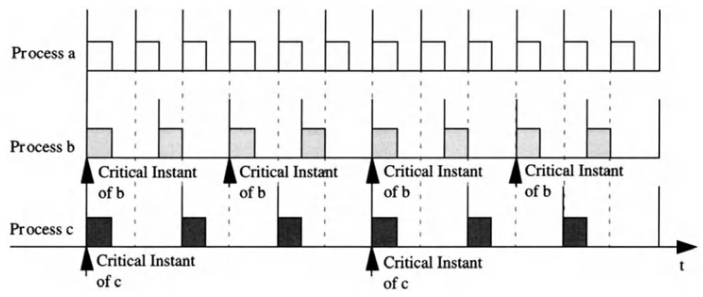
\includegraphics[width=0.8\textwidth]{critical-instants}
	\caption{Example of critical instants.}\label{fig:critical-instants}
\end{figure}
%--------------------------Figure end -------------------


%%%%%%%%%%%%%%%%%%%%%%%%%%%%%%%%%%%%%%%%%%
%%										%
%%				FIGURE				   	%
%%										%
%%%%%%%%%%%%%%%%%%%%%%%%%%%%%%%%%%%%%%%%%%
%\begin{figure}[H]
%	\centering
%	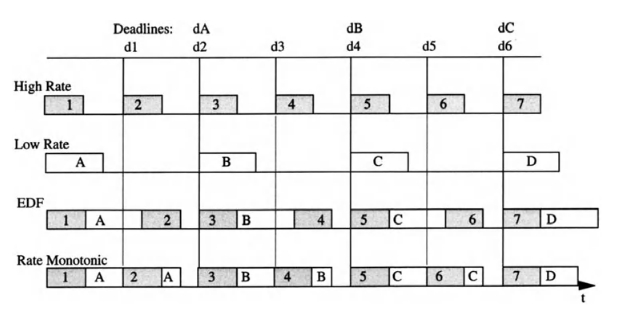
\includegraphics[width=\textwidth]{edf-vs-rate}
%	\caption[Rate monotonic versus EDF]{Rate monotonic versus EDF: context switches in preemptive systems.}{\label{fig:edf-vs-rate}}
%\end{figure}
%%--------------------------Figure end -------------------

\subsection{System Architecture}
The employment of continuous media in multimedia systems also imposes additional, new requirements to the system architecture. The audio and video data need to be copied directly from adapter to adapter for acquiring the shortest possible path. A problem with direct copying from adapter to adapter is the control and the change of quality of service parameters. In multimedia systems, such an adapter to adapter connection is defined by the capabilities of the two involved adapters and the bus performance. This architecture of low-level data streaming corresponds with proposals for using additional new busses for audio and video transfer within a computer. It also enables a switch-based rather than a bus-based transfer within a computer.

The architecture of the protocol processing system is just one issue to be considered in the system architecture of multimedia supporting operating systems. Multimedia data should be delivered from the input device (e.\ g.\ CD-ROM) to an output device (e.\ g.\ a video decompression board) across the fastest possible path. The paradigm of streaming from source to sink is an appropriate way of doing this. Hence, the multimedia application opens devices, establishes a connection between them, starts the data flow and returns to other duties.


The most dominant characteristic of multimedia applications is to preserve the temporal requirement at the presentation time. Therefore, multimedia data is handled in a \textit{Real-Time Environment (RTE)}, i.\ e.\ , its processing is scheduled according to the inherent timing requirements of multimedia data. On a multimedia computer, the RTE will usually coexist with a \textit{Non-Real-Time Environment (NRTE)}. The NRTE deals with all data that have no timing requirements. Figure \ref{fig:rte-nrte} shows the approached architecture.


%%%%%%%%%%%%%%%%%%%%%%%%%%%%%%%%%%%%%%%%%
%										%
%				FIGURE				   	%
%										%
%%%%%%%%%%%%%%%%%%%%%%%%%%%%%%%%%%%%%%%%%
\begin{figure}[ht!]
	\centering
	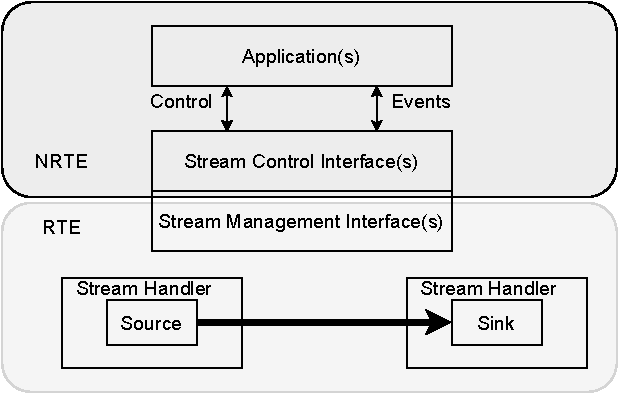
\includegraphics[width=0.8\textwidth]{rte-nrte}
	\caption{Real-time and non-real-time environments.}\label{fig:rte-nrte}
\end{figure}
%--------------------------Figure end -------------------

Multimedia I/O devices are, in general, accessed from both environments. Data such as a video frame, for example, is passed from the RTE to the display. The RTE is controlled by related functions in the NRTE. The establishment of communication connections at the start of a stream must not obey timing requirements, but the data processing for established connections is compelled. All control functions are performed in the NRTE. 

System programs, such as communication protocol processing and database data transfer programs, make use of this programming in the RTE. Whereas applications like authoring tools and media presentation programs are relieved from the burden of programming in the RTE, they just interface and control the RTE services. Applications determine processing paths which are needed for their data processing, as well as the control devices and paths.

To reduce data copying, buffer management functions are employed in the RTE. This buffer management is located ``between'' the stream handlers. Stream handlers are
entities in the RIE which are in charge of multimedia data.

Multimedia data usually ``enters'' the computer through an input device, a source and ``leaves" it through an output device, a sink (where storage can serve as an I/O
device in both cases). Sources and sinks are implemented by a device driver.
%\subsubsection{UNIX-based Systems}
%In the UNIX operating system, the applications in the user space generally make use of system calls in the NRTE. Either the whole operating system or a part of it is also located in the NRTE and in the kernel space. Extensions to the operating system providing real-time capabilities make up the RTE part of the kernel space (see Figure \ref{fig:rte-nrte-unix}).
%
%
%%%%%%%%%%%%%%%%%%%%%%%%%%%%%%%%%%%%%%%%%%%
%%%										%
%%%				FIGURE				   	%
%%%										%
%%%%%%%%%%%%%%%%%%%%%%%%%%%%%%%%%%%%%%%%%%%
%\begin{figure}[ht!]
%	\centering
%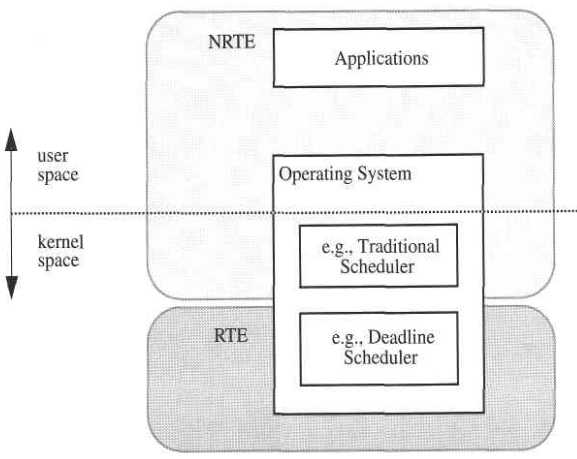
\includegraphics[width=0.8\textwidth]{rte-nrte-unix}
%\caption{NRTE and RTE In UNIX systems.}{\label{fig:rte-nrte-unix}}
%\end{figure}
%
%%-------------------FIGURE END---------------------------
%The actual implementation of the RTE varies substantially:
%\begin{itemize}
%	\item SUN OS includes real-time static priorities and provides a RTE.
%	
%	\item AIX includes real-time priorities. This feature provides the basis for the RTE in the AIX-based UltimediaTM server.
%		
%	\item The IRIX operating system on Silicon Graphics Workstations has real-time capabilities, i.e., it includes an RTE.
%	
%	\item Linux OS has partitioning of priority space into static real-time and dynamic priorities, hence allowing RTE. Different implementations of SRT schedulers may use either static real-time or dynamic priority mechanisms.
%\end{itemize}
%
%\subsubsection{QuickTime}
%QuickTime is a software extension to the Macintosh System. It provides the capability
%to capture, store, manage, synchronize and display continuous media data. A more
%detailed description can be found in [DM92]. It introduces digitized video as standard
%data type into the system, and it allows an easier handling of other continuous media
%like audio and animation. Standard applications are enhanced by multimedia capabili-
%ties. Apple has announced QuickTime to be available for other operating systems like
%Windows and UNIX as well. An integration of future hardware and software
%developments is possible.
%
%The standard data type of QuickTime is a movie. All kinds of continuous media
%data are stored in movie documents. Additionally, time information like the creation
%and modification date, duration, etc., are also kept in the movie document. With each
%movie, a poster frame is associated that appears in the dialog box. Other information
%like current editing selection, spatial characteristics (transformation matrix, clipping
%region) and a list of one or more tracks are associated with the movie. A track repre-
%sents a stream of information (audio or video data) that flows in parallel to every other
%track. With each track, information like creation and modification data, duration, track
%number, spatial characteristics (transformation matrix, display window, clipping
%region), a list of related tracks, volume and start time, duration, playback rate and a data
%reference for each media segment is stored. A media segment is a set of references to
%audio and video data, including time information (creation, modification, duration),
%language, display or sound quality, media data type and data pointers. Future releases
%will have, apart from audio and video tracks, "custom tracks" such as a subtitle track.
%All tracks can be viewed or heard concurrently. The tracks of a movie are always syn-
%chronized. Since movies are documents they cannot only be played (including pausing,
%stepping through, etc.), but they can also be edited. Operations like cut, copy and paste
%are possible. Movie documents can be part of other documents. QuickTime is scalable.
%Hardware components like accelerator or compressor/decompressor cards can be
%employed.
%
%The QuickTime architecture comprises three major components (see Figure 3-9):
%the Movie Toolbox offers a set of services to the user that allows himlher to incorporate
%movies into applications. These applications may directly manipulate characteristics of
%audio and video data of movies. The movie is integrated in the desktop environment.
%Movie data can be imported and exported with the system clipboard and a movie can be
%edited within the Movie Toolbox.
%
%The second component, known as the Image Compression Manager, provides a
%common interface for compression and decompression of data, independent of the
%implementation, to and from hard disk, CD-ROM and floppy. It offers a directory ser-
%vice to select the correct compression component. Different interface levels for differ-
%ent application requirements are available. The compression techniques are a
%proprietary image compression scheme, a JPEG implementation and a proprietary
%video compressor for digitized video data (leading to a compression ratio of 8:1, and if
%temporal redundancies are also removed, to a ratio of 25: 1).
%
%%%%%%%%%%%%%%%%%%%%%%%%%%%%%%%%%%%%%%%%%%
%%										%
%%				FIGURE				   	%
%%										%
%%%%%%%%%%%%%%%%%%%%%%%%%%%%%%%%%%%%%%%%%%
%\begin{figure}[H]
%	\caption{QuickTime architecture}{\label{fig:quciktime-arch}}
%\end{figure}
%
%%-------------------FIGURE END---------------------------
%
%An Animation Compressor can compress digital data in lossy and lossless (error-free)
%modes. A graphics compressor is also available. The pixel depth conversion in bits per
%pixel can be used as a filter to be applied in addition to other compressors.
%
%The Component Manager provides a directory service related to the components.
%It is the interface between the application and various system components. It shields
%developers from having to deal with the details of interfacing with specific hardware. In
%the Component Manager, object-oriented concepts (e.g., hierarchical structure, extensi-
%ble class libraries, inheritance of component functionality, instance-based client/server
%model) are applied. Thus, applications are independent of implementations, can easily
%integrate new hardware and software and can adapt to the available resources. The com-
%ponents managed by the Component Manager are the Clock, the Image Compressor
%and Image Decompressor, the Movie Controller, the Sequence Grabber, Sequence
%Grabber Channel and the Video Digitizer. Furthermore, application-defined compo-
%nents can be added.
%
%There is a simple resource management scheme applied to the local environment
%only: in the case of scarce resources, audio is prioritized over video, i.e., audio playback
%is maintained (if possible) whereas single video frames might be skipped. If an applica-
%tion calls the Movie Toolbox during playback, there are the following possibilities to
%handle these calls:
%
%\begin{itemize}
%	\item The commonly used mode is a preemptive calling sequence, where the application
%	returns to the system after each update. This might cause jerky movie output.
%	\item With a non-preemptive calling sequence, the application does not return to the
%	system while a movie is played. This counteracts the multitasking capability.
%	\item The high-performance controlled preemptive calling sequence is a compromise,
%	where the application gives up control to the Movie Toolbox for a specified time
%	period (e.g., 50 ms).
%\end{itemize}
%
%
%As an additional resource management scheme for better performance, it is recom-
%mended to tum off the virtual memory while playing QuickTime movies. If it is on, it
%will cause the sound to skip and it will lower the frame rate during the playback of a
%movie. However, no RTE exists.
%
%The concept of components in QuickTime allows for easy extension without
%affecting applications. It attempts to form a hierarchical structure of functionality by
%components. The movie controller component eases user interface programming. A
%disadvantage of QuickTime is that there is no clear layering of abstractions for
%programmers and that the functionality of managers and components sometimes
%overlaps.
%
%
%\subsubsection{Windows Multimedia Extensions}
%The Microsoft Windows Multimedia Extensions (WME) are an enhancement to the
%Windows programming environment. They provide high-level and low-level services
%for the development of multimedia applications for application developers, using the
%extended capabilities of a multimedia personal computer [Win91].
%The following services for multimedia applications are provided by the WME:
%
%
%\begin{itemize}
%	\item A Media Control Interface (MCI) for the control of media services. It comprises
%	an extensible string-based and message-based interface for communication with
%	MCI device drivers. The MCI device drivers are designed to support the playing
%	and recording of waveform audio, the playing of MIDI (Musical Instrument Digi-
%	tal Interface) file, the playing of compact disk audio from a CD-ROM disk drive
%	and the control of some video disk players.
%	
%	\item A Low-level API (Application Programming Interface) provides access to multi-
%	media-related services like playing and recording audio with waveform and MIDI
%	audio devices. It also supports the handling of input data from joysticks and
%	precise timer services.
%	
%	\item A multimedia file I/O service provides buffered and unbuffered file 110. It also
%	supports the standard IBMIMicrosoft Resource Interchange File Format (RIFF)
%	files. These services are extensible with custom 110 procedures that can be shared
%	among applications.
%	
%\item The most important device drivers available for multimedia applications are:
%
%\begin{itemize}
%	\item An enhanced high-resolution video display driver for Video 7 and Paradise
%	VGA cards providing 256 colors, improved performance, and other new
%	features.
%	\item A high-resolution VGA video display driver allowing the use of a custom 16-
%	color palette as well as the standard palette.
%	\item A low resolution VGA video display driver providing 320-by-320 resolution
%	with 256 colors.
%	\item The Control Panel Applets that allow the user to change display drivers, to
%	set up a screen saver, to install multimedia device drivers, to assign wave-
%	form sounds to system alerts, to configure the MIDI Mapper and to calibrate
%	joysticks. A MIDI Mapper supports the MIDI patch service that allows
%	MIDI files to be authored independently of end-user MIDI synthesizer
%	setups.
%\end{itemize}
%\end{itemize}
%
%Figure \ref{fig:wme-arch} shows the rough architecture of MS Windows Multimedia Extensions:
%MMSYSTEM library provides the Media Control Interface services and low-level mul-
%timedia support functions. The communication between the low-level MMSYSTEM
%functions and multimedia devices, such as waveform, MIDI, joystick and timer, is
%provided by the multimedia device drivers. The high-level control of media devices is
%provided by the drivers for the Media Control Interface.
%
%
%%%%%%%%%%%%%%%%%%%%%%%%%%%%%%%%%%%%%%%%%%
%%										%
%%				FIGURE				   	%
%%										%
%%%%%%%%%%%%%%%%%%%%%%%%%%%%%%%%%%%%%%%%%%
%\begin{figure}[H]
%	\caption{MS Windows Multimedia Extensions architecture}{\label{fig:wme-arch}}
%\end{figure}
%
%%-------------------FIGURE END---------------------------
%
%The main concepts of the architecture of the Multimedia Extensions are extensibility
%and device-independence. They are provided by a translation layer (MMSYSTEM) that
%isolates applications from device drivers and centralizes device-independent code, run-
%time linking that allows the MMSYSTEM translation layer to link to the drivers it
%needs and a well-defined and consistent driver interface that minimizes the
%development of specialized code and makes the installation and upgrade processes
%easier.
%
%Current Microsoft Windows platforms provide many advanced technologies,
%based on underlying multimedia system architectures for media streaming and media
%processing, to run and display applications rich in multimedia elements such as full-
%color graphics, video, 3-D animation and surround sound. Some of the technologies are
%the Microsoft DirectX, Windows Media, Microsoft DirectShow, and others.


%%%%%%%%%%%%%%%%%%%%%%%%%%%%%%%%%%%%%%%%%%%

%  Multimedia Communication System       %

%%%%%%%%%%%%%%%%%%%%%%%%%%%%%%%%%%%%%%%%%%%


\section{Multimedia Communication System}
From the communication perspective, we divide the higher layers of the Multimedia Communication System (MCS) into two architectural subsystems: an \textit{application subsystem} and a \textit{transport subsystem}.

\subsection{Application Subsystem}
\subsubsection{Collaborating Computing}
Infrastructure of networked workstations and PCs, and the availability of audio and video at these end-points, makes it easier for people to cooperate and bridge \textit{space} and \textit{time}. In this way, network connectivity and end-point integration of multimedia provides users with a \textit{collaborative computing} environment. Collaborative computing is generally known as \textit{Computer-Supported Cooperative Work} (CSCW).
		
There are many tools for collaborative computing, such as:
\begin{multicols}{2}
	\begin{itemize}
		 \item \textit{electronic mail}, 
		 \item \textit{internet relay chat (IRC)}, 
		 \item \textit{forums},
		 \item \textit{screen sharing tools}, 
		 \item \textit{text-based conferencing systems}, 
		 \item \textit{telephone conference systems}, 
		 \item \textit{conference rooms} and 
		 \item \textit{video conference systems}.
	\end{itemize}
\end{multicols}


We present a framework for collaborative computing and general related issues exemplified by different systems and tools.	

\subsubsection*{Collaborative Dimensions}	
Electronic collaboration can be categorized according to three main parameters:
\begin{multicols}{3}
	\begin{itemize}
		\item \textit{time}
		\item \textit{user scale} and 
		\item \textit{control}
	\end{itemize}
\end{multicols}


Therefore, the collaboration space can be partitioned into a three-dimensional space (shown in Figure {\ref{fig:cola-dim}}).

%%%%%%%%%%%%%%%%%%%%%%%%%%%%%%%%%%%%%%%%%
%										%
%				FIGURE				   	%
%										%
%%%%%%%%%%%%%%%%%%%%%%%%%%%%%%%%%%%%%%%%%
\begin{figure}[ht!]
	\centering
	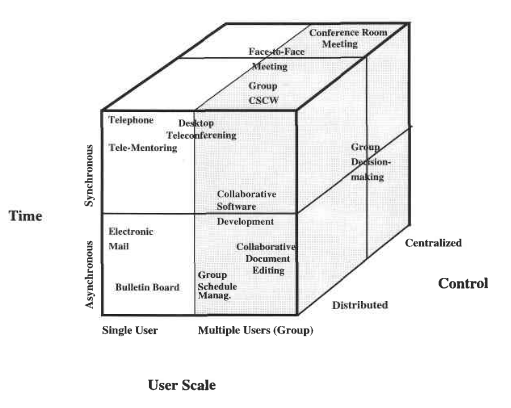
\includegraphics[width=0.8\textwidth]{cola-dim}
	\caption{Dimensions of collaborative computing.}\label{fig:cola-dim}
\end{figure}
%--------------------------Figure end -------------------


\paragraph*{Time}
With respect to time, there are two modes of cooperative work: \textit{asynchronous} and \textit{synchronous}:
\begin{itemize}
	\item \textit{Asynchronous cooperative} work specifies processing activities
	that do not happen at the same time.
	\item The \textit{synchronous cooperative} work happens at the same time.
\end{itemize}

\paragraph*{User Scale}
The user scale parameter specifies whether a \textit{single user} collaborates with
another user or a \textit{group} of more than two users collaborate together. Groups can
be further classified as follows:

\begin{itemize}
	\item A group may be \textit{static} or \textit{dynamic} during its lifetime:
	\begin{itemize}
		\item A group is \textit{static} if its participating members are predetermined and membership does not	change during the activity.
		\item A group is \textit{dynamic} if the number of group members varies during the collaborative activity, i.\ e.\ , group members can join or leave the activity at any time.
	\end{itemize}
	\item Group members may have different roles in the Computer-Supported Cooperative Work (CSCW), e.\ g.\ a \textit{member} of a group, a \textit{participant} of a group activity, a \textit{conference initiator}, a \textit{conference chairman}, a \textit{token holder} or an \textit{observer}.
	
	\item Groups may consist of members which have homogeneous or heterogeneous characteristics and requirements of their collaborative environment.
\end{itemize}

\paragraph*{Control}
 Control during the collaboration can be \textit{centralized} or \textit{distributed}
\begin{itemize}
	\item \textit{Centralized} control means that there is a chairman (e.\ g.\ main manager) who controls the collaborative work and every group member (e.\ g.\ user agent) reports to him or her. 
	
	\item \textit{Distributed} control means that every group member has control over his/her
	own tasks in the collaborative work and distributed control protocols are in place
	to provide consistent collaboration.
\end{itemize}

\paragraph{Group Communication Architecture}

Group communication (GC) includes the synchronous or asynchronous communication of several users under central or distributed control. 

An architectural model for this communication comprises:
\begin{itemize}
	\item a support model, 
	\item a system model, and 
	\item an interface model.
\end{itemize}

The support model includes group \textit{communication agents}, which communicate over a network (see Figure \ref{fig:group-communication-architecture}). These agents include individual components, each dedicated to special aspects:


\begin{figure}[pht]
	\centering
	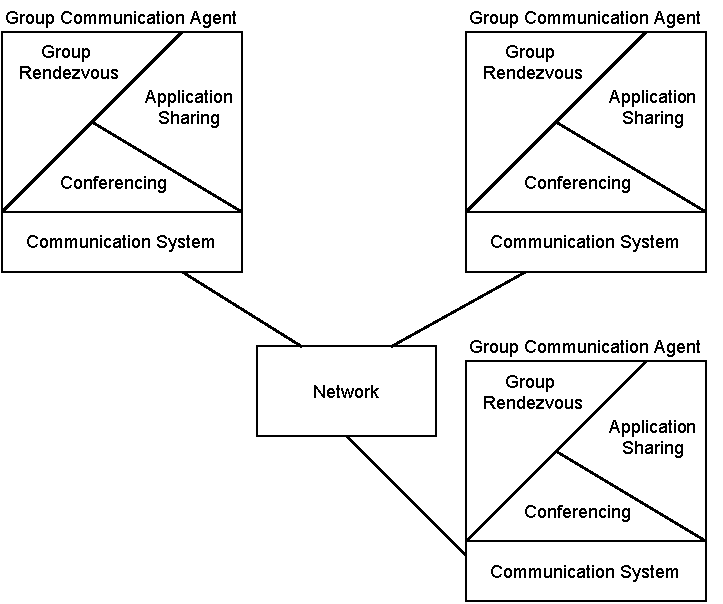
\includegraphics[width=0.7\textwidth]{group-communication-architecture}
	\caption{Group communication support model.}
	\label{fig:group-communication-architecture}
\end{figure}

\begin{itemize}
	\item \textbf{Group Rendezvous}
	Group rendezvous denotes a method which allows one to organize meetings, and to get information about the group, ongoing meetings and other static and dynamic information.
	
	\item \textbf{Shared Applications}
	Application sharing denotes techniques which allow one to replicate information to multiple users simultaneously. The remote users may point to interesting aspects (e.\ g.\, via tele-pointing) of the information and modify it so that all users can immediately see the updated information (e.\ g.\, joint editing). Shared applications mostly belong to collaboration-transparent application.
	
	\item \textbf{Conferencing}
	Conferencing is a simple form of collaborative computing. This service provides the management of multiple users for communicating with each other using multiple media. Conferencing applications belong to collaboration-aware applications.
\end{itemize}

The GC system model is based on a client-server model. 
\begin{itemize}
	\item \textbf{Clients} provide user interfaces for smooth interaction between group members and the system. 
	
	\item \textbf{Servers} supply functions for accomplishing the group communication work, and each server specializes in its own function.
\end{itemize}


The GC interface model includes two kinds of protocols for exchanging information within the GC support model:
\begin{enumerate}
	\item \textbf{User presentation protocols}
	User presentation protocols perform interactions among the clients, such as opening a conference, closing a conference, dynamic joining and leaving of a meeting and floor passing.
	
	\item \textbf{Group work management protocols}
	 Group work management protocols specify the communication between the clients and the servers. Services such as registration of active conferences and queries for further conference information are supported by these protocols.
	
\end{enumerate}


\subparagraph{Group Rendezvous}
Group rendezvous denotes a method which allows one to organize meetings, and to get information about the group, ongoing meetings and other static and dynamic information. There are \textit{synchronous} and \textit{asynchronous} methods for group rendezvous:

\begin{itemize}
	\item \textbf{Synchronous Rendezvous Methods}
	\begin{itemize}
		\item These methods use directory services and explicit invitations. 
		\item Directory	services access information stored in a knowledge base about the conference,
		such as the name of the conference, registered participants, authorized users and name and role of the participants.
		\item The explicit invitations method sends invitations either point-to-point or point-to-multipoint to conference participants.
	\end{itemize}

\item \textbf{Asynchronous Rendezvous Methods}
	\begin{itemize}
		\item These methods may be implemented through e-mail or bulletin boards. 
		\item The e-mail based mechanism encapsulates in the body message enough information about a group session establishment.
		\item Bulletin boards on the internet announces seminars, classes, conferences and other open meetings of a school or institution.
	\end{itemize}
\end{itemize}

\subparagraph{Applications Sharing}
Sharing applications is recognized as a vital mechanism for supporting group communication activities.
\begin{itemize}
	\item Sharing applications means that when a shared application program (e.\ g.\ editor) executes any input from a participant, all execution results performed in the shared object (e.\ g.\ document text) are distributed among all the participants. 
\end{itemize}

An important issue in application sharing is shared control. The primary design decision in sharing applications is to determine whether they should be \textit{centralized} or \textit{replicated}:

\begin{itemize}
	\item \textbf{Centralized Architecture}
	\begin{itemize}
		\item In a centralized architecture, a single copy of the shared application runs at
		one site. 
		\item All participants' input to the application is forwarded to the local site and the application’s output (shared object) is then distributed to all	sites.
		\item The advantage of the centralized approach is \textit{easy maintenance} because there is only one copy of the application that updates the shared object.
		\item The disadvantage is \textit{high network traffic} because the output of the application needs to be distributed every time.
	\end{itemize}
	
	\item \textbf{Replicated Architecture}
	\begin{itemize}
		\item In a replicated architecture, a copy of the shared application runs locally at each site. 
		\item Input events to each application are distributed to all sites and	each copy of the shared application is executed locally at each site.
		\item The Advantages of this architecture are:
		\begin{itemize}
			\item \textit{Low network traffic}, because only input events are distributed among the sites.
			\item \textit{Low response times}, since all participants get their output from local copies of the application.
		\end{itemize}
	\item The disadvantages are:
	\begin{itemize}
		\item The requirement of \textit{the same execution environment} for the application at each site, and 
		\item The \textit{difficulty in maintaining consistency}. 
	\end{itemize}
	\end{itemize}
\end{itemize}

Figure \ref{fig:centralized-arch} shows centralized architecture and Figure \ref{fig:replicated-arch} shows replicated architecture.
\begin{figure}[tph]
	\centering
	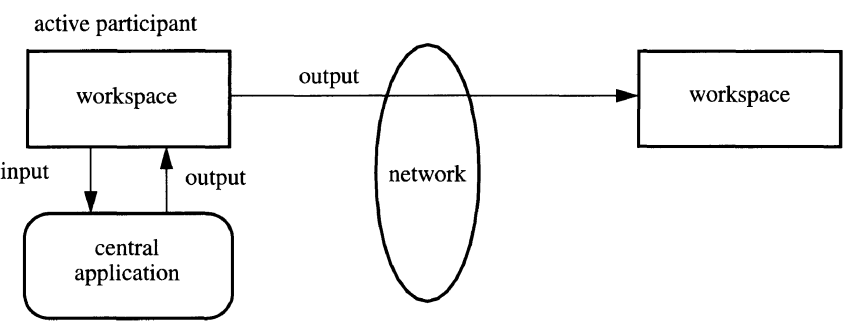
\includegraphics[width=0.7\textwidth]{graphics/centralized-arch}
	\caption{Centralized architecture.}
	\label{fig:centralized-arch}
\end{figure}

\begin{figure}[bph]
	\centering
	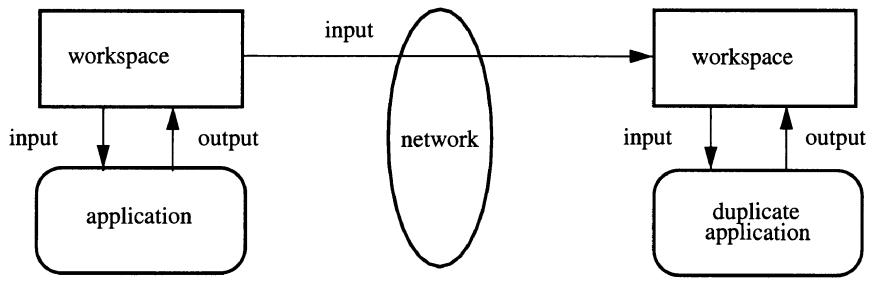
\includegraphics[width=0.7\textwidth]{graphics/replicated-arch}
	\caption{Replicated architecture.}
	\label{fig:replicated-arch}
\end{figure}


The abstraction of a \textit{floor} is used to ensure consistency of distributed data objects (e.\ g.\ multimedia documents), or applications (programs) shared among participants. Only one member of the group, namely the one who currently owns the floor, called the \textit{floor holder}, has the right to manipulate distributed objects within the shared workspace. The floor holder is the only user who can create input events for the shared application, i.\ e.\ , modify data, which will then be available to all users.

A possible shared data manipulation architecture is shown in Figure \ref{fig:shard-data-arch}. 
\begin{itemize}
	\item A CSCW control component resides at every-site and dispatches input events coming from an 	input device (e.\ g.\ , keyboard, mouse). 
	\item The control component checks whether the system is currently used by the set of floor holders. 
	\item If this is the case, then the inputs are accepted locally and processed, and then	passed on to the other systems.
	\item If the local system is not a floor holder, then the local	inputs are rejected by the control component.
	\item However, the control component accepts input events transmitted by other participating systems.
\end{itemize}


\begin{figure}[th!]
	\centering
	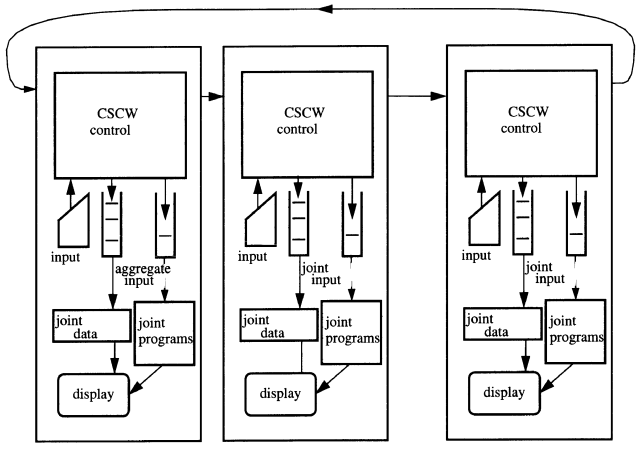
\includegraphics[width=0.7\textwidth]{shard-data-arch}
	\caption{Shared data manupulation architecture.}
	\label{fig:shard-data-arch}
\end{figure}


\subparagraph{Conferencing}
Conference supports collaborative computing and is also called synchronous tele-collaboration. Conferencing is a management service that controls the communication among multiple users via multiple media, such as video and
audio, to achieve simultaneous face-to-face communication.


More precisely, video and audio have the following purposes in a teleconferencing system:

\begin{itemize}
	\item \textit{Video} is used in technical discussion to display view-graphs and to indicate	how many users are still physically present at a conference. For visual support, workstations, PCs or video walls can be used.
	\item \textit{Audio} is used for describing and	clarifying visual information. Therefore, quality audio, with true full-duplex communication and echo cancellation, and possibly enhanced with spatial queues, is necessary.
\end{itemize}

Conference control includes several functions:
\begin{itemize}
	\item \textit{Establishing} a conference, where the conference participants agree upon a	common state, such as identity of a chairman (moderator), access rights (floor control) and audio encoding. Conference systems may perform
	registration, admission, and negotiation services during the conference	establishment phase.
	\item \textit{Closing} a conference.
	\item \textit{Adding} new users and removing users who leave the conference.
\end{itemize}

Conference states can be stored (located) either on a central machine (centralized control), where a central application acts as the repository for all information related to the conference, or in a distributed fashion. The control model follows from the location of the conference state. Accordingly, the control model may be either \textit{centralized} or \textit{distributed}.

\begin{itemize}
	\item \textbf{Centralized Conference Control}
	\begin{itemize}
		\item Centralized conference control means that the conference is set up at one central location. 
		\item An initiator opens the conference by selecting and explicitly inviting an initial group of participants.
		\item This means that the initiator needs to know the addresses of all conference participants.
	\end{itemize}
\item \textbf{Distributed Conference Control}
\begin{itemize}
	\item Distributed conference control is based on a distributed conference state. 
	\item This state is	achieved as follows: 
	\begin{itemize}
		\item The initiator of the conference selects one or several multicast addresses for the transmission of information to the participants, and opens the conference. 
		\item Conference participants can join by responding to the receipt of special multicast data. 
		\item The announcement information (multicast address, port) required for this purpose is previously sent or made available to the participants by use of the group rendezvous protocols.
	\end{itemize}
\end{itemize}
\end{itemize}

\subsubsection{Session Management}
Session management is the core part which separates the control, needed during the transport, from the actual transport.

\paragraph{Architecture}
A session management architecture is built around and \textit{entity-session} manager which separates the control from the transport. By creating a reusable session manager, which is separated from the user-interface, conference-oriented tools avoid a duplication of their effort. A possible session control architecture is shown in Figure \ref{fig:session-control-arch}. The session control architecture consists of the following components:

%%%%%%%%%%%%%%%%%%%%%%%%%%%%%%%%%%%%%%%%%
%										%
%				FIGURE				   	%
%										%
%%%%%%%%%%%%%%%%%%%%%%%%%%%%%%%%%%%%%%%%%
\begin{figure}[ht]
	\centering
	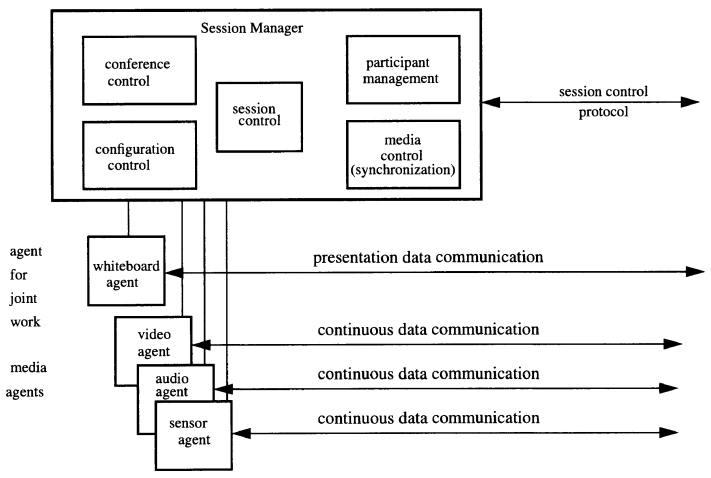
\includegraphics[width=0.8\textwidth]{session-control-arch}
	\caption{Example of session control architecture.}\label{fig:session-control-arch}
\end{figure}
%--------------------------Figure end -------------------

\subparagraph{Session Manager}
	Session managers assume \textit{local} and \textit{remote} functions. Local functions include:
		\begin{enumerate}
			\item membership control management, such as participant authentication or presentation of coordinated user interfaces;
			\item control management for shared workspace, such as \textit{floor control};
			\item media control management, such as intercommunication among media agents or synchronization;
			\item \textit{configuration management}, such as exchange of interrelated QoS parameters or selection of appropriate services according to QoS; and
			\item \textit{conference control management}, such as an establishment, modification and a closing of a conference.
		\end{enumerate}
	
\textit{Remote} functions include the communication with other session managers to exchange status information, which may include floor information and configuration information.
	
\subparagraph{Media Agents}	
Media agents are separate from the session manager, and they are responsible for decisions specific to each type of media. 
\begin{itemize}
	\item This modularity allows a replacement of agents. 
	\item Each agent performs its own control mechanism over the particular medium, such as mute, unmute, change video quality, start sending, stop sending, etc.
\end{itemize}


\subparagraph{Shared Workspace Agent}
The shared workspace agent transmits shared objects (e.\ g.\ telepointer coordinate, graphical or textual object) among the shared applications.

\paragraph{Session Control}
Each session is described by its \textit{session state}. The state information (name of the session, start, valid policies) is either \textit{private} (e.\ g.\ , local resources), or \textit{shared} by all participants.

Session management includes two steps to process the session state: an \textit{establishment}
and a \textit{modification} of the session. During the establishment, the session manager
negotiates, agrees, and sets the logical state of its own session. It negotiates and defines the transport topology with the transport subsystem. 

Mechanisms embedded in session management:

\subparagraph{Floor/Activity Control}
		\begin{itemize}
	\item Within shared workspaces, the floor control is employed to provide access to
	the shared workspace.
	\item Further, the floor control in shared applications is often used to maintain data consistency.
	\item Floor control, applications use a \textit{floor-passing mechanism} (gavel-passing, chalk-passing).
	\item The floor-passing mechanism means that at any time, only one
	participant has the floor. 
	\item The floor is handed off to another participant when
	requested. 
	\item To obtain the floor, the participant must explicitly take action to
	signal a floor change
\end{itemize}

\subparagraph{{Conference Control}}
For conferencing applications, conference control is employed.
	 
\subparagraph{{Media Control}}	 
Media control mainly includes a functionality, such as the synchronization of media stream.

\subparagraph{{Configuration Control}}
Configuration control includes a control of media quality, QoS handling, resource availability and other system components to provide a session according to users requirements.

\subparagraph{{Membership Control}}
Membership control may include services, for example, \textit{invitation}, on to a session, \textit{registration} into a session, \textit{modification} of the membership during the session,
etc.

\subsection{Transport Subsystem}
\subsubsection{Requirements}
Networked multimedia applications by themselves impose new requirements onto data handling in computing and communications because they need:
\begin{multicols}{2}
\begin{enumerate}
	 \item substantial data throughput,  
	 \item fast data forwarding,  
	 \item service guarantees, and 
	 \item multicasting.
\end{enumerate}
\end{multicols}


\paragraph{Data Throughput}
\begin{itemize}
	\item Audio and video data resemble a stream-like behavior, and they demand, high \textit{data throughput}. 
	\item In a workstation or network, several of those streams may exist concurrently, demanding a high throughput.
\end{itemize}

\paragraph{{Fast Data Forwarding}}
Fast data forwarding imposes a problem on end-systems where different applications exist in the same end-system, and they each require data movement ranging from normal, error-free data transmission to new time-constraint traffic types transmission. 

\paragraph{{Service Guarantees}}
	Distributed multimedia applications need service guarantees, otherwise their acceptance does not come through as these systems, working with continuous media, compete against analog radio and television services.

\paragraph{{Multicasting}}
	Multicast is important for multimedia-distributed applications in terms of sharing resources like the network bandwidth and the communication protocol processing at end-systems. 



\subsubsection{Transport Layer}
Transport protocols serve to support addressing of communication end-points within end-systems, 
%\begin{multicols}{2}
	\begin{itemize}
		\item \textit{fragmentation} and \textit{reassembly} of data, 
		\item \textit{flow} and \textit{congestion control},\textit{error control}, as well as 
		\item \textit{connection  establishment} and \textit{closure}.
	\end{itemize}
%\end{multicols}



Transport protocols, to support multimedia transmission, need to have new features and provide the following functions: 
\begin{multicols}{2}
	\begin{itemize}
		\item timing information 
		\item semi-reliability 
		\item multicasting 
		\item NAK (None-AcKnowledgment)-based \textit{error recovery mechanism} and 
		\item rate control
	\end{itemize}
\end{multicols}


The Internet protocol stack includes two types of transport protocols:

\paragraph{Transmission Control Protocol (TCP)}
	
Early implementations of video conferencing applications were implemented on top of	the TCP protocol. 
\begin{itemize}
	\item TCP provides a reliable, serial communication path, or virtual circuit, between processes exchanging a full-duplex stream of bytes.
	\item Each process is assumed to reside in an Internet host that is identified by an IP address. 
	\item Each process has a number of logical, full-duplex ports through which it can set up and use full-duplex TCP connections.
	\item During the data transmission over the TCP connection, TCP must achieve \textit{reliable}, \textit{sequenced delivery} of a stream of bytes by means of an underlying, unreliable IP datagram service. 
	\item To achieve this, TCP makes use of re-transmission on time-outs and positive acknowledgments upon receipt of information.
	\item Because re-transmission can cause both out-of-order arrival and duplication of data, sequence numbering is crucial.
\end{itemize}

Flow control in TCP makes use of a window technique in which the receiving side of the connection reports to the sending side the sequence numbers it may transmit at any	time and those it has received contiguously thus far.
	
For multimedia, the \textit{positive acknowledgment} causes substantial overhead as all	packets are sent with a fixed rate. \textit{Negative acknowledgment} would be a better strategy. Further, TCP is not suitable for real-time video and audio transmission because its re-transmission mechanism may cause a violation of deadlines which disrupt the continuity of the continuous media streams. TCP was designed as a transport protocol suitable for non-real-time reliable applications, such as file transfer, where it performs the best.





\paragraph{User Datagram Protocol (UDP)}
UDP is a simple extension to the Internet network protocol IP that supports multiplexing of datagrams exchanged between pairs of Internet hosts. It offers only \textit{multiplexing} and \textit{checksums}, nothing else. Higher-level protocols using UDP must provide their own retransmission, packetization, reassembly, flow control, congestion avoidance, etc.

Many multimedia applications use this protocol because it provides some degree of real-time transport property, although loss of PDUs may occur. For experimental purposes, UDP above IP can be used as a simple, unreliable connection for medium transport.

In general, UDP is not suitable for continuous media streams because it does not provide the notion of connections, at least at the transport layer; therefore, different service guarantees cannot be provided.


\paragraph{Real-time Transport Protocol (RTP)}
RTP is an end-to-end protocol providing network transport functions suitable for applications transmitting real-time data, such as audio, video or simulation data over multicast or unicast network services. RTP is primarily designed to satisfy the needs of multi-party multimedia conferences, but it is not limited to that particular application. RTP provides functions, such as:
\begin{multicols}{2}
	\begin{itemize}
		\item determination of media encoding
		\item synchronization, framing
		\item error detection
		\item encryption
		\item timing and
		\item source identification
	\end{itemize}
\end{multicols}



\paragraph{Xpress Transport Protocol (XTP)}
XTP was designed to be an efficient protocol, taking into account the low error ratios and higher speeds of current networks. XTP integrates transport and network protocol functionalities to have more control over the environment in which it operates.

It defines six service types: 
\begin{multicols}{2}
	\begin{enumerate}
		\item connection
		\item transaction
		\item unacknowledged datagram
		\item acknowledged datagram
		\item isochronous stream and
		\item bulk data
	\end{enumerate}
\end{multicols}



\subsubsection{Network Layer}
The requirements on the network layer for multimedia transmission are a provision of \textit{high bandwidth}, \textit{multicasting}, \textit{resource reservation} and \textit{QoS guarantees}, \textit{new routing protocols} with support for streaming capabilities and new \textit{higher-capacity routers} with support of integrated services.	

\subsubsection*{IP}

\paragraph[IPv4]{Internet Protocol Version 4 (IPv4)}
IP provides for the unreliable transfer of datagrams from a source host to destination hosts, possibly passing through one or more gateways (routers) and networks in the process. Following are the IP properties:
\begin{enumerate}
	\item \textit{Types of Service}
	\item \textit{Addressing and Multicasting}
	\item \textit{Interconnectivity Between Internet Protocol and Underlying Networks}
	\item \textit{Routing}
\end{enumerate}

\subparagraph{Types of Service}
IP includes identification of the service quality through the Type of Service (TOS) specification. TOS specifies:
\begin{enumerate}
	\item precedence relation and
	\item services such as \textit{minimize delay},
	\textit{maximize throughput}, \textit{maximize reliability},\textit{ minimize monetary cost} and \textit{normal service}.
\end{enumerate}


\subparagraph{Addressing and Multicasting}
One of the most critical functions of the IP is the \textit{addressing}, i.\ e.\ , to establish a global address space that allows every network on the Internet to be uniquely identified. The IP	addressing structure is shown in Figure \ref{fig:ipv4-addressing}.

The network addressing structure was revised to accommodate five classes of address: $ A $, $ B $, $ C $, $ D $ and $ E $
\begin{itemize}
	\item Class $ A $ retained the $ 24bits $ host identifier field, but only $ 7bits $ for	network number. This address space covers a small number of class $ A  $ networks. 
	
	\item Class	$ B $ with $ 16 bits $ for the host identifier and $ 14 bits $ for the network number allows a larger number of Class $ B $ networks. 
	\item Class $ C $ allocates $ 21 bits $ for network number and $ 8bits $ for host identifier, therefore many more Class $ C $ networks are available. 
	
	\item Class $ D $ addresses, are used for \textit{multicasting}.
	\item Class $ E $ addresses have been reserved for future extensions.
\end{itemize}
%%%%%%%%%%%%%%%%%%%%%%%%%%%%%%%%%%%%%%%%%
%										%
%				FIGURE				   	%
%										%
%%%%%%%%%%%%%%%%%%%%%%%%%%%%%%%%%%%%%%%%%
\begin{figure}[pht]
	\centering
	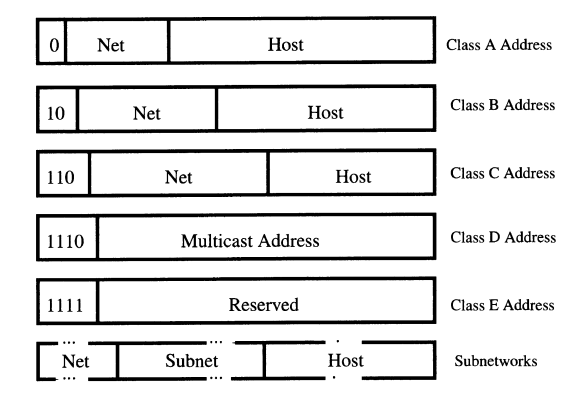
\includegraphics[width=0.8\textwidth]{ipv4-addressing}
	\caption{IPv4 addressing structure.}\label{fig:ipv4-addressing}
\end{figure}
%--------------------------Figure end -------------------


\subparagraph{Interconnectivity Between Internet Protocol and Underlying Networks}
The Internet family of protocols is one of today's most widespread protocol stacks in computer networking. There is a strong interest in transporting the IP datagrams, which may carry multimedia traffic, over different networks, for example, Ethernet, ATM B-ISDN, MPLS, or \texttt{IEEE 802.11} wireless networks. Hence, the mapping between the Internet protocol and the underlying layers is of importance. Another important function in this task is the binding of IP addresses to lower-level network addresses.


\subparagraph{Routing}
A major subject in Internet architecture is the routing of IP packets because the basic	model of Internet consists of networks connected by routers. To create an opportunity for further experimental exploration of different routing protocols for global networking, the concept of \textit{Autonomous Systems} (AS) was developed. ASs are collections of routers falling under a common administrative authority. In theory, the routers commonly use the same routing protocol- Interior Gateway Protocol (IGP), within the AS.	AS of gateways (routers) exchange reachability information by means of an Exterior Gateway Protocol (EGP).

As the common IGP for the Internet, the \textit{Open Shortest Path First} (OSPF) has been adopted.

Another IGP protocol is the \textit{Routing Information Protocol} (RIP). RIP was one of	the first routing protocols used with IP and was implemented by the program routed that comes with most UNIX systems.

RIP uses a \textit{distance vector} algorithm to propagate routing information. A router running RIP advertises the destinations it can reach along	with a distance to each destination; adjacent routers receive the information and update heir routing tables.

For EGP, the \textit{Border Gateway Protocol} (BGP) was developed. BGP allows the sender and receiver to enforce policies, to provide facilities for transit routing, and it uses TCP for all communication to ensure	reliable transport.
	
\paragraph[IPv6]{Internet Protocol Version 6 (IPv6)}
\begin{itemize}
	\item One of the major reasons why a new version of IP protocol is considered is the \textit{limited address space} of IPv4. 
	\item Second major motivation for changes in IP have arisen from new Internet applications such as audio and video applications.
	\item Third motivation is that IPv4 is fully missing security functions.
\end{itemize}


IPv6 retains many of the design features that have made IPv4 successful. Hence, IPv6 is also connectionless protocol, where each datagram contains a destination address, and each datagram is routed independently. Despite retaining the basic concepts from the current version, IPv6 changes can be categorized as follows: 

		\begin{enumerate}
		\item enhanced addressing and improved routing, 
		\item simplification of IP header format, 
		\item improved support of IP options, 
		\item support of QoS, 
		\item support of security, and 
		\item fragmentation of data.
	\end{enumerate}


\begin{framed}
	\begin{itemize}
		\item IPv6 utilizes 128-bit Internet addresses. Therefore, it can support $ 2^{128} $ Internet addresses.
		
		\item IPv6 is represented by 8 sets of 4 hexadecimal digits separated by colon.
		Example: \texttt{2001:db8:85a3:0000:0000:8a2e:370:7334}
		
		
		\item For example: the above IPv6 address can be represented as
		\texttt{2001:db8:85a3::8a2e:370:7334}
		
		Here are 6 sets of hexadecimal 4 digits number so :: represents two sets of \texttt{0000} within it.
	\end{itemize}
\end{framed}


\paragraph[IGMP]{Internet Group Management Protocol (IGMP)}
IGMP is a protocol for managing Internet multicasting groups. It is used by conferencing applications to join and leave particular multicast group. The basic service permits a source to send datagrams to all members of a multicast group. There are no guarantees of the delivery to any or all targets in the group.

A multicast router periodically sends queries (Host Membership Query messages) with a Time-to-Live (TTL) value of 1 (in order not to leave the connected LAN segment) to refresh their knowledge of memberships present on a particular network. If there exist multiple multicast routers on that network segment, one of them will be
responsible to respond to the query

\paragraph[RSPV]{Resource reServation Protocol (RSPV)}
RSVP is a protocol which transfers reservations and keeps a state at the intermediate nodes. It does not have a data transfer component. RSVP messages are sent as IP datagrams, and the router keeps ``soft state'', which is refreshed by periodic reservation messages. In the absence of the refresh messages, the routers delete the reservation after a certain timeout.

This protocol was specified by IETF to provide one of the components for integrated services on the Internet. To implement integrated services, four components need to be implemented: 
\begin{enumerate}
	\item the packet scheduler, 
	\item admission control routine, 
	\item classifier, and 
	\item the reservation setup protocol.
\end{enumerate}


RSVP reservations\footnote{A reservation specifies the amount of resources to be reserved for all, or some subset of the packets in a particular session.} are receiver-oriented, which means that the sender starts, but the actual reservation of resources is performed by the receiver. This is done to support heterogeneous receivers in a multicast group.


\subsection{Quality of Service and Resource Management}
 Quality of service is the ability to provide different priorities to different applications, users, or data flows, or to guarantee a certain level of performance to a data flow. 

The user/application requirements on multimedia systems need to be mapped into services which then make the effort to satisfy the requirements. Due to the heterogeneity of requirements, services in multimedia systems must be parameterized. The result is the \textit{``quality-controllable services"} which then allow to classify and differentiate system and communication services.

Parameterization of services was defined first in ISO (International Standard Organization) standards through the notion of Quality of Service (QoS). The ISO standard defined QoS as a concept for specifying how \textit{``good"} the offered networking services are.

\emph{Quality of Service indicates the defined and controlling behavior of a service expressed through quantitative measurable parameter(s)}.

\subsubsection*{QoS Layering}
Traditional QoS (ISO standards) was defined by the network layer of the communication system. An enhancement of QoS was achieved through inducing QoS into transport services. For Multimedia Communication System (MCS), the QoS notion must be extended because many other services contribute to the end-to-end service quality.

The MCS consists of three layers: 
\begin{itemize}
	\item \textit{application}, 
	\item \textit{system} (including communication services and operating system services), and 
	\item \textit{devices} (network and Multimedia (MM) devices). 
\end{itemize}

Above the application may or may not reside a human user. This implies the introduction of QoS in the application (application QoS), in the system (system QoS) and in the network (network QoS). In the case of having a human user, the MCS may also have a user QoS specification. We concentrate in the network layer on the network device and its QoS because it is of interest to us in the MCS. The MM devices find their representation (partially) in application QoS. 

%%%%%%%%%%%%%%%%%%%%%%%%%%%%%%%%%%%%%%%%%
%										%
%				FIGURE				   	%
%										%
%%%%%%%%%%%%%%%%%%%%%%%%%%%%%%%%%%%%%%%%%
\begin{figure}[pht]
	\centering
	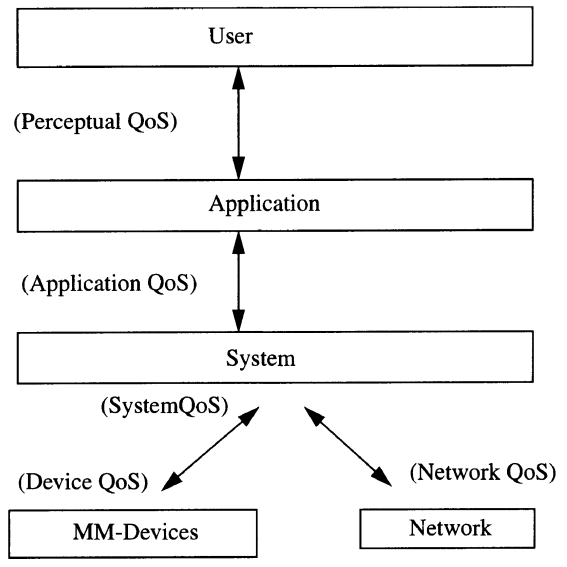
\includegraphics[width=0.6\textwidth]{qos-layer}
	\caption{QoS-layered model for the MCS.}\label{fig:qos-layer}
\end{figure}
%--------------------------Figure end -------------------

\paragraph*{Perceptual/User QoS} 
The \textit{perceptual QoS} parameters need to allow for description of two major requirements:
\begin{itemize}
	\item description of \textbf{perceptive qualities} such as media quality (e.\ g.\ ,	excellent, good, or bad quality), windows size (e.\ g.\ , big, small), response time (e.\ g.\ , interactive, batch), security (e.\ g.\ , high, low), and 
	\item description of \textbf{pricing choices}, i.\ e.\, users should be able to specify the range of price they are willing to pay for the desired	service.
\end{itemize}

\paragraph*{Application QoS}
Application QoS parameters describe requirements for application services in terms of:
\begin{itemize}
	\item \textbf{media quality}, including media characteristics (e.\ g.\ , frame rate, frame resolution), and their transmission characteristics (e.\ g.\ , end-to-end delay, jitter); 
	
	\item \textbf{media relations}, specifying relations among media (e.g., media transformation, inter and intra frame synchronization skews); and
	
	\item \textbf{adaptation rule}s (e.\ g.\ , actions if network bandwidth is scare).
\end{itemize}


\paragraph*{System QoS}
System QoS parameters describe requirements, placed on communication and computing services, derived from application QoS. They may be specified in terms of \textit{quantitative} and \textit{qualitative} criteria. 
\begin{itemize}
	\item \textbf{Quantitative criteria} represent concrete measures such as \textit{bit per second}, \textit{number of errors}, \textit{task processing time}, \textit{task period}. 
	\begin{itemize}
		\item The QoS parameters include then \textit{throughput}, \textit{delay}, \textit{response time},\textit{ data rate}, \textit{data corruption} at the system level, task and \textit{buffer specifications}. 
	\end{itemize}
		\item \textbf{Qualitative criteria} specify the expected functions needed for provision of QoS such as \textit{interstream} \textit{synchronization}, \textit{ordered data delivery},\textit{ error-recovery mechanisms}, \textit{scheduling mechanisms} and others.
\end{itemize}

\paragraph*{Network QoS}
Network QoS parameters describe requirements, placed on low level network services. They may be specified in terms of:
\begin{itemize}
	\item \textbf{network load}, describing the ongoing	network traffic and characterized through average/minimal interarrival time on the network connection, burstiness, packet/cell size and service time in the node for a connection's packet/cell and
	
	\item \textbf{network performance}, describing network service guarantees. Performance might be expressed through a source to destination delay bound for a packet, or packet loss rate, or others.
\end{itemize}

\paragraph*{Device QoS}
Device QoS parameters typically specify timing and throughput demands for media data units given by audio/video devices.

\subsubsection*{QoS Parameter Values and Types of Service}
The specification of QoS parameter values determines the type of service, called \textit{service class}. There are at least three service classes:
\begin{enumerate}
	\item guaranteed, 
	\item predictive and best
	\item effort services.
\end{enumerate}

\paragraph*{Guaranteed Services} 
Guaranteed services provide QoS guarantees, as specified through the QoS parameter values either in \textit{deterministic} or \textit{statistical} representation. 
\begin{itemize}
	\item The \textit{deterministic} values can be given through a single value (e.\ g.\ average value, threshold value, target value), a pair of values (e.\ g.\ minimum and average value, lowest quality and target quality) or an	interval of values (lower bound and upper bound). 
	\item \textit{Statistical} value specifies statistical bound on error rate etc. 
\end{itemize}

\paragraph*{Predictable Services}
A predictive service is based on past network behavior, hence the QoS parameters are estimates of past behavior which the service tries to match.

\paragraph*{Best Effort Services}
Best-effort services are based on either no guarantees, or on partial guarantees. There is either no specification of QoS parameters required, or some bounds in deterministic or statistical forms are given.

\subsubsection[Resource Management]{Resource Management Architecture}
Resources are managed by various components of a resource management subsystem in a networked multimedia system (Figure \ref{fig:resource-mgmt}). The main goal of resource management is to provide guaranteed delivery of multimedia data. This goal implies three main actions: 
\begin{enumerate}
	\item to \textit{reserve} and allocate resources (end-to-end) during multimedia call establishment so that traffic can flow according to the QoS specification, which means distribution and negotiation of the QoS specification for system components involved in the data transfer from the source(s) to the sink(s);
	
	\item to \textit{provide} resources according to the QoS specification, which means adhering to resource allocation during multimedia delivery using proper service disciplines; and
	
	\item to \textit{adapt} to resource changes during ongoing multimedia data processing.
\end{enumerate}
The resource management subsystem includes \textit{resource managers} at the hosts as well as the network nodes. \textit{Resource management protocols} are used to exchange information about resources among the resource management. 


%%%%%%%%%%%%%%%%%%%%%%%%%%%%%%%%%%%%%%%%%
%										%
%				FIGURE				   	%
%										%
%%%%%%%%%%%%%%%%%%%%%%%%%%%%%%%%%%%%%%%%%
\begin{figure}[pht]
	\centering
	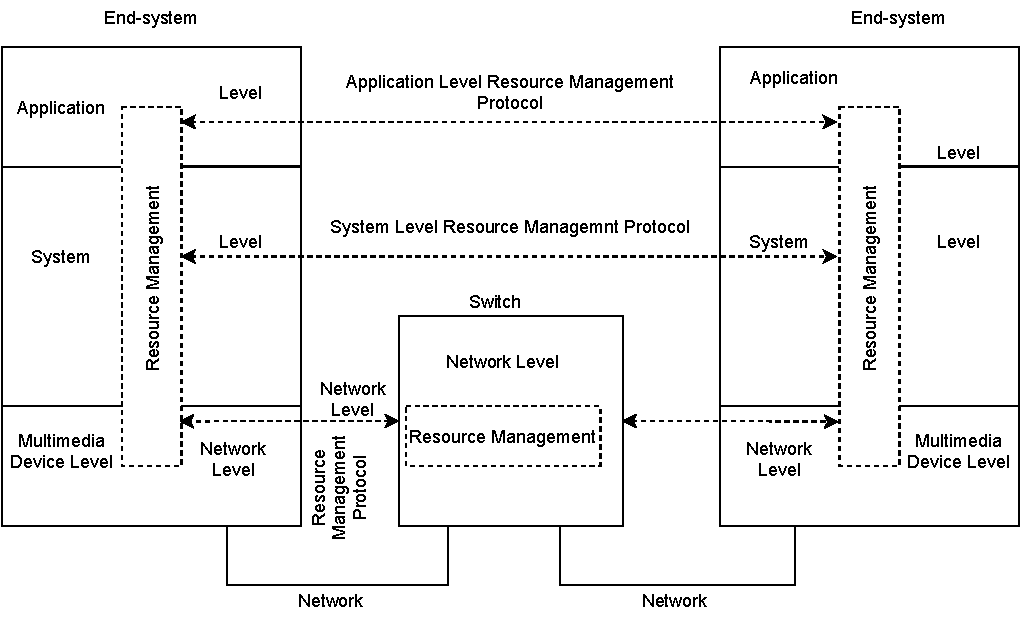
\includegraphics[width=\textwidth]{resource-mgmt}
	\caption{Resource management in MCSs.}\label{fig:resource-mgmt}
\end{figure}
%--------------------------Figure end -------------------


\subsubsection*{Relation Between QoS and Resources}

The requested output QoS parameters are dependent on:
\begin{itemize}
	\item the \textit{input quality}, 
	\item the \textit{resource capacity} allocated to services (processes), and 
	\item the \textit{scheduling algorithms} managing the shared resources for the distributed multimedia system.
\end{itemize}
 

According to the requested output QoS parameters, we can determine how much resources are required to achieve it. 
\begin{itemize}
	\item For example, the requested end-to-end delay parameter determines the behavior of transmission services along the path between media source and sink with respect to:
	\item packet scheduling (bandwidth allocation),
	\item queueing (buffer allocation) and 
	\item task scheduling (CPU allocation).
\end{itemize}


The above described relation between QoS and resources can be expressed in the form of different mappings, service curves, and profiles. The relation between QoS and
resources is established in two phases:

\begin{enumerate}
	\item \textit{Establishment Phase} (Setup) and
	\item \textit{Runtime Phase} (Enforcement)
\end{enumerate}

%Description of a possible realization of resource allocation and management shows the QoS and resource relation. Consider resource allocation and management based on the interaction between clients and their respective resource managers. The client requests a resource allocation by specifying its requirements through a QoS specification (this implicitly includes a mapping between the QoS specification and the required resources). This is equivalent to a workload request. The resource manager checks its own resource utilization and decides if the reservation request can be served or not. All existing reservations are stored, this way their share in terms of the respective resource capacity is guaranteed. Moreover, this component negotiates the reservation request with other resource managers if necessary.


\paragraph*{Establishment Phase}
As shown in Figure \ref{fig:establishment-phase}, resources are reserved (planned) and allocated during the connection setup according to the QoS specification. 
\begin{multicols}{2}
	\begin{enumerate}
		\item This means that during the establishment, an application client requests a resource allocation by specifying its requirements through an application QoS specification. 
		\item This QoS specification is then translated by a QoS translator entity (e.\ g.\ , QoS compiler) into the system QoS specification and their required resources.
		\item The required resources represent then the reservation request to the resource	management. 
		\item The resource management checks the resource utilization and decides if the reservation request can be served. 
		\item If the reservation can be granted along the end-to-end path, a QoS contract is provided to the application/user. 
		\item If reservation cannot be granted, the request is rejected.
	\end{enumerate}
\end{multicols}


\begin{figure}[tph]
	\centering
	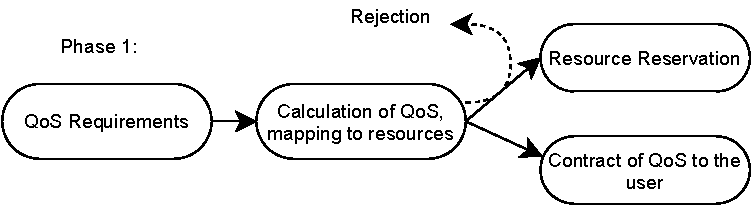
\includegraphics[width=0.7\textwidth]{graphics/establishment-phase}
	\caption{Establishment phase.}
	\label{fig:establishment-phase}
\end{figure}



\paragraph*{Runtime Phase}
As shown in Figure \ref{fig:runtime-phase},  resources must be provided according to QoS specifications during the lifetime of an application. 

\begin{multicols}{2}
	\begin{enumerate}
		\item This means, that once the resource reservation and allocation are performed during the establishment phase, the QoS enforcement must occur during the runtime phase. 
		\item The resource allocation must be enforced through mechanisms such as traffic shaping and appropriate scheduling mechanisms. 
		\item If any changes in resource allocation occur, an adaptation needs to be in place to adjust the data transfer if necessary.
	\end{enumerate}
\end{multicols}


\begin{figure}[tph]
	\centering
	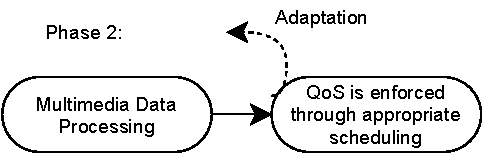
\includegraphics[width=0.6\textwidth]{runtime-phase}
	\caption{Runtime phase.}
	\label{fig:runtime-phase}
\end{figure}



%%%%%%%%%%%%%%%%%%%%%%%%%%%%%%%%%%%%%%%%%

%		Abstraction of programming      %

%%%%%%%%%%%%%%%%%%%%%%%%%%%%%%%%%%%%%%%%%

\section{Abstraction of Programming}
\subsection{Abstraction Levels}

%%%%%%%%%%%%%%%%%%%%%%%%%%%%%%%%%%%%%%%%%
%										%
%				FIGURE				   	%
%										%
%%%%%%%%%%%%%%%%%%%%%%%%%%%%%%%%%%%%%%%%%
\begin{figure}[ht!]
	\centering
	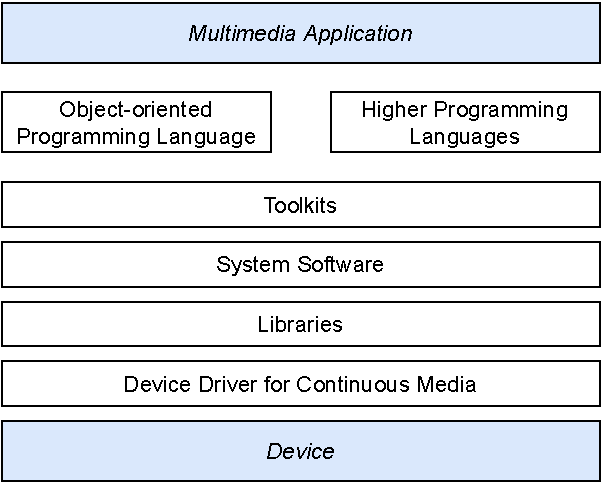
\includegraphics[width=0.6\textwidth]{abstraction-level}
	\caption{Abstraction levels of the programming of multimedia systems.}\label{fig:abstraction-level}
\end{figure}
%--------------------------Figure end -------------------


\begin{multicols}{2}
		\textit{Abstraction levels} in programming define different approaches with a varying degree of detail for representing, accessing and manipulating data. A multimedia application may access each level.	
		
		A \textit{device} for processing continuous media can exist as a separate component in a computer. In this case, a device is not part of the operating system, but is directly accessible to every component and application. 
		
		A \textit{library}, the simplest abstraction level, includes the necessary functions for controlling the corresponding hardware with specific device access operations.
		
		As with any device, multimedia devices can be bound through a device driver, respectively the operating system. Hence, the processing of the continuous data becomes part of the \textit{system software}.
		
		Multimedia \textit{device drivers} embedded in operating systems simplify considerably the implementation of device access and scheduling.
		
		\textit{Higher procedural programming languages} build the next abstraction level. They are the languages most often used to implement commercial multimedia applications. Further, they can contain abstractions of multimedia data. The code generated from the compiler can be processed through libraries, as well as through a system interface for continuous data.
		
		More flexibility for the programmer is provided via the abstraction level - \textit{an object-oriented environment}. This environment provides the application with a class hierarchy for the manipulation of multimedia. Also in this case, the generated or interpreted code can be processed and controlled through libraries, as well as through a system interface for continuous media (see Figure {\ref{fig:abstraction-level}}).
	
\end{multicols}

\subsection{Libraries}

\begin{multicols}{2}
	\begin{itemize}
		\item The processing of continuous media is based on a set of functions which are embedded into libraries. 
		\item This is the usual solution for programming multimedia data. 
		\item These libraries are provided together with the corresponding hardware.
		\item Some libraries can be considered as extensions of the graphical user interface, whereas other libraries consist of control instructions passed as control blocks to the corresponding driver.
	\end{itemize}
\end{multicols}
	

\subsection{System Software}
Instead of implementing access to multimedia devices through individual libraries, the device access can become part of the operating system. An example of access to multimedia devices and support for continuous media processing implemented in operating system is the experimental \textit{Nemo} system from the University of Cambridge. 

%The Nemo system consists of the Nemo Trusted Supervisor Call, running in supervisor mode, and three domains running in user mode: \textit{system}, \textit{device driver} and \textit{application}.	
	
%The \textit{Nemo Trusted Supervisor Call (NTSC)} code implements those functions which are required by user mode processes. It provides support for three types of processes. System processes implement the majority of the services provided by the operating system. Device driver processes are similar to system processes, but are distinguished by the fact that they are attached to device interrupt stubs which execute in supervisor mode. Application processes contain user programs. Processes interact with each other via the system abstraction - \textit{InterProcess Communication} (IPC) - which is implemented using low-level system abstractions \textit{events} and, if required, \textit{shared memory}. These system abstractions support the continuous media communication among processes.	

%The NTSC calls are separated into two classes, one containing calls which may only be executed by a suitable privileged system process such as kernel, the other containing calls which may be executed by any process. Further, NTSC is responsible for providing an interface between a multimedia hardware device and its associated driver process. This device driver implementation ensures that if a device has only a low-level hardware interface to the system software, code can be implemented within a device driver stub to implement a higher level interface. This allows the system builder to trade off hardware complexity and cost against the processor cycles required to implement a high-level device interface.

\subsection{Toolkits}
A simpler approach for control of the audio and video data processing can be taken by using \textit{toolkits}. These toolkits are used to:

\begin{itemize}
	\item Abstract from the actual physical layer.
	\item Allow a uniform interface for communication with all different devices of continuous media.
	\item Introduce the client-server paradigm.
\end{itemize}	
	
Toolkits can also hide process-structures. It is possible to embed toolkits into the programming languages or object-oriented environment.
	
\subsection{Higher Programming Languages}

\begin{multicols}{2}
	\begin{itemize}
		\item In HLL, the processing of continuous media data is influenced by a group of similar constructed functions. 
		\item These calls are mostly hardware and driver-independent. 
		\item Hence, their integration in HLLs leads to a wishful abstraction, supports a better programming style and increases the productivity.
		\item The programs in an HLL either directly access multimedia data structures, or communicate directly with the active processes in a real-time environment. 
		\item The processing devices are controlled through corresponding device drivers. 
		\item Compiler, linker and/or loader provide the required communication between the application program and the processing of continuous data. 
	\end{itemize}
\end{multicols}

Media can be considered differently inside a programming language.


\begin{multicols}{2}
	\subsubsection{Media as Types}
	\begin{itemize}
		\item One of the alternatives to programming in an HLL with libraries is the concept of \textit{media as types}.
		\item Here, the data types for video and audio are defined.
		\item In the case of text, character is the type (the smallest addressable element).
		\item A program can address such characters through functions and sometimes directly through operators. 
		\item They can be copied, compared with other characters, deleted, created, read from a file or stored. 
		\item Further, they can be displayed, be part of other data structures, etc.
	\end{itemize}
\end{multicols}

. 
\subsubsection{Media as Files}
	Another possibility of programming continuous media data is the consideration of continuous media streams as \textit{files instead} of data types.
\begin{lstlisting}
	file_h1 = open(MICROPHONE_1,...)
	file_h2 = open(MICROPHONE_2,...)
	file_h3 = open(SPEAKER, ...)
	...
	read(file_h1)
	read(file_h2)
	mix(file_h3, file_h1, file_h2)
	activate(file_h1, file_h2, file_h3)
	...
	deactivate(file_h1, file_h2, file_h3)
	...
	rc1 = close(file_h1)
	rc2 = close(file_h2)
	rc3 = close(file_h3)\end{lstlisting}

The example describes the merging of two audio streams. The physical file is associated during the open process of a file with a corresponding file name. The program receives a \textit{file descriptor} through which the file is accessed. In this case, a device unit, which creates or processes continuous data streams, can be associated with a file name.	

\textit{Read} and \textit{write} \textit{functions} are based on continuous data stream behavior. Therefore, a new value is assigned continuously to a specific variable which is connected, for example, with one read function. On the other hand, the read and write functions of discrete data occur in separate steps. For each assignment of a new value from a file to the corresponding variable, the read function is called again.

An \textit{activate function} means that the actual data transmission starts and a deactivate function means that the transmission stops.

\subsubsection{Media as Processes}
The processing of continuous data contains a time-dependency because the life span of a process equals to the life span of a connection(s) between source(s) and destination(s). A connection can exist locally, as well as remotely.

\begin{lstlisting}
PROCESS cont_process_a;
	...
	On_message_do
		set_volume ...
		set_loudness ...
		...
	...
	[main]
pid = create (cont_process_a)
send(pid, set_volume, 3)
send(pid, set_loudness)
...
\end{lstlisting}
In the above example, the process \texttt{cont\_process\_a} implements a set of \textit{actions} (\textit{functions}) which apply to a continuous data stream, Two of them are the modification
of the volume \texttt{set\_volume} and the process of setting a volume, dependent from a band filter, \texttt{set\_loudness}.

\subsubsection{Programming Language Requirements}
The processing of continuous data is:
	\begin{itemize}
		\item Controlled by the HLL through pure asynchronous instructions.
		\item An integral part of a program through the identification of the media, respectively data streams with data types, variables, files or processes.
	\end{itemize}

Therefore, the HLL should support a \textit{parallel processing}.

\begin{multicols}{2}
	\subsection{Object-oriented Approaches}
	\begin{itemize}
		\item The object-oriented approach was first introduced as a method for the reduction of complexity in the software development and it is used mainly with this goal today.
		\item Further, the reuse of software components is a main advantage of this paradigm. 
		\item The basic ideas of object-oriented programming are: \textit{data encapsulation} and \textit{inheritance}, in connection with \textit{class} and \textit{object} definitions. 
		\item Instead of using functions and data structures, programs are implemented by using classes, objects, and methods.
	\end{itemize}
\end{multicols}



\begin{multicols}{2}
	\subsubsection{Abstract Type Definition}
	\begin{itemize}
		\item The definition of data types through abstract interfaces is called \textit{abstract type definitions}. 
		\item The abstract type definition is understood as an interface specification without a knowledge and implementation of internal algorithms. 
		\item This data abstraction hides the used algorithm.
		\item In a distributed multimedia system, abstract data types are assumed for virtual and real device units such as cameras and monitors. 
	\end{itemize}
\end{multicols}



\begin{multicols}{2}
	\subsubsection{Class}
	\begin{itemize}
		\item The implementation of abstract data types is done through classes. 
		\item A class specification includes an interface provided to the outside world.
		\item For example, in a class \textit{professional camera}, the operations \textit{zoom} and \textit{set back-light} are defined and implemented. 
		\item If the objects, which represent a closed class, use only relative position entries, the implementation of the \textit{zoom} operation needs to transform the absolute values into the necessary relative parameters.
	\end{itemize}
\end{multicols}




\begin{multicols}{2}
	\subsubsection{Object}
	\begin{itemize}
		\item An \textit{object} is the instance of the class. 
		\item Therefore, all objects, derived from the same class include the same operations as an interface to the outside world. 
		\item An object is created at run-time of the system. 
		\item It includes a set of operations, which are called \textit{methods}. 
		\item Additionally, each object has an \textit{internal state}, which exists during the life span of the object, but it can only be accessed using the methods associated with this object.
		\item It can be compared with a global variable assigned to a process, but not with local variables of functions and procedures.
		\item Objects communicate among each other through the exchange of messages. 
		\item Thus, a \textit{message} calls the corresponding method of the target object.
	\end{itemize}
\end{multicols}
In a distributed multimedia environment, virtual units are considered to be objects. Multimedia data units (the LDU's images, audio and video clips) can also be considered objects.


\subsubsection{Inheritance}
One of the most important properties of object-oriented systems is inheritance.  Classes contain, besides the root and leaves of the hierarchy, super classes and subclasses (parent and child).
\begin{multicols}{2}
	\begin{itemize}
		\item For example, let the class \textit{professional-camera} be a subclass of the class \textit{camera}. 
		\item Methods such as \textit{autofocus-on} and \textit{focus} are defined in the class \textit{camera}. 
		\item The \textit{professional-camera} class also has the method \textit{zoom}. 
		\item An object, which is derived from the \textit{professional-camera}, can use the method \textit{zoom}, as well as the operations \textit{focus} and, \textit{autofocus-on}.
	\end{itemize}
\end{multicols}
The main problem has been and remains to be the design of a clear and uniform class hierarchy for a multimedia system.

%Until now, only simple inheritance was considered. For example, for the application interface of a conference application, it is not possible to explicitly combine all necessary devices for each conference. Such an application would be dependent on a certain set ofdevice types which are bound together in the required configuration. Device binding often includes different basic devices. A conference object inherits properties of different objects in an object-oriented environment, therefore a multi-inheritance is often useful.


\subsubsection{Polymorphism}

\begin{multicols}{2}
Polymorphism is related to the property of inheritance indicating when the same name of a method is defined in several classes (and objects) with different implementations and functionalities. 
	\begin{itemize}
		\item For example, the function play is used with audio and video data. 
		\item It uses different device units for each medium. 
		\item The data can come either from a file of a local file environment or from an audio-video sequence of an external device. 
		\item Inside the object-oriented approach, for example, play is defined in different classes. 
		\item According to which object must perform the operation, the corresponding method is chosen.
\end{itemize}
\end{multicols}

The complexity of different types and device units is reduced and there is a common set of method names for classes and objects of different media.  On the other hand, polymorphism can also very easily cause programming errors that are difficult to find. Hence, this abstraction strongly complicates the implementation. This can occur easily
through unwanted, multiple identical method names.

%%%%%%%%%%%%%%%%%%%%%%%%%%%%%%%%%%%%

%	Synchronization					%

%%%%%%%%%%%%%%%%%%%%%%%%%%%%%%%%%%%%
\section{Synchronization}
\subsection{Introduction}
Synchronization is the coordination of the events to operate a system in unison. Systems operating with all their parts in synchrony are said to be synchronous or in sync. Synchronization in multimedia systems refers to the temporal relations between media objects in the multimedia system. Synchronization between media objects comprises	relations between time-dependent media objects and time-independent media objects. It is addressed and supported by many system components including the operating system, communication system, databases, and documents and even often by applications.
	
%The Merriam-Webster Dictionary defines the term	synchronization as follows:
%
%	Synchronization = the act or result of synchronizing; the state of being synchronous.
%%	
%	Synchronize = to happen at the same time; to represent or arrange (events) to indicate coincidence or coexistence; to make synchronous in operation; to make (motion picture sound) exactly simultaneous with the action.
%	
%	Synchronization creates a relationship between independent objects (pieces of informa-
%	tion, media, processes, data streams, LDUs). Synchronization between media objects
%	includes relationships between time-dependent and time-independent objects. An
%	example for synchronization of continuous media from everyday life is the synchroni-
%	zation of visual and acoustic information in television broadcasting. A multimedia sys-
%	tem has to produce a similar synchronization for audio and motion picture information.
%	An example for temporal relationships of time-dependent and time-independent media
%	is a slide show. The representation of the slides is synchronized to the commented audio
%	stream. To implement a slide show in a multimedia system, we have to synchronize the
%	playback of pictures to the relevant sections of the audio stream.
%	
%	In multimedia systems, there are the three relationships between two or more
%	objects that occur most frequently; we will explain them below. Figure 8-1 represents a
%	schematic view of these relationships.
%	
%	%%%%%%%%%%%%%%%%%%%%%%%%%%%%%%%%%%%%%%%%%
%	%										%
%	%				FIGURE				   	%
%	%										%
%	%%%%%%%%%%%%%%%%%%%%%%%%%%%%%%%%%%%%%%%%%
%	\begin{figure}[H]
%		\caption{Relationships bewtween data units}\label{fig:wme-arch}
%	\end{figure}
%	
%	%-------------------FIGURE END---------------------------
%	
%\textbf{	Content Relationships} These relationships define a connection between various
%	media objects or data. For example, a content relationship in a document could exist
%	between the data in a table and a relevant picture. The data is represented in various
%	ways (table or picture), or various aspects of an interrelated fact are presented. In such a
%	desirable form of integrated documents, the input data, the links, and the type of pre-
%	sentation are defined or edited. All actual output data resulting from the representation
%	of linked input data (in this example the table and a picture) cannot be directly changed
%	or edited. If input data is changed, then this can have various effects on the output data
%	in different places of the document. Techniques to maintain consistency are known
%	from database systems and could be transferred to the range of different media in multi-
%	media systems. In general, an implementation of content relationships origins from
%	common data structures. The presentation can be in various media, but it always
%	expresses a consistent fact.
%	
%	\textbf{Spatial Relationships} These relationships are normally called layout relationships;
%	they define the space for the representation of a media object from an output device of a
%	multimedia presentation at a specific point in time. In two-dimensional output devices
%	(e.g., monitor or paper), the layout defines the two-dimensional area to be used.
%	
%	These relationships are important for the presentation on paper and monitor. They
%	determine the layout in the user interface: The objects are arranged in a two-dimen-
%	sional space to each other. Here, purely spatial information is significant. In desktop
%	publishing documents, this is usually expressed in frames. Aframe is inserted and con-
%	tents are assigned to the frame. Such frames can also be used to insert motion pictures.
%	Windows systems use several windows for this purpose. A window can offer the reader
%	additional degrees of freedom by use of operations like "zoom in", "zoom out", or
%	"move". Holographic experiments and three-dimensional projections onto surfaces
%	allow also an arrangement on a third dimension (the depth), which Windows systems
%	show only in a rudimentary overlapping. Descriptive attributes include cascade and tile.
%	Note that spatial references can exist even in the presentation of audio, when using the
%	stereo effect [LCP90]. In a workstation conference, several participants can be acousti-
%	cally arranged. To produce a direct reference to single images or motion pictures of the
%	other persons, the video windows are represented in the same spatial arrangement on
%	the monitor. This technique has a positive effect on the acceptance of an application,
%	i.e., the users can follow a discussion in a more natural way. Without acoustic place-
%	ment, the speaker can be identified only by recognizing his or her voice, by the
%	contents, or by his or her lip movements.
%	
%\textbf{	Temporal Relationships} These relationships define time relationships between
%	media objects. They are important whenever there are time-dependent media objects.
%	
%	A temporal relationship like "play back at the same time" is significant, particu-
%	larly when viewing time-specific media. For example, the playback of motion pictures
%	and sound should be correlated in terms of time. The temporal reference between objects represents synchronization in the true sense of the word. Descriptive attributes
%	include concurrent, independent, or consecutive.
%	
%	The synchronization relationships across several spaces have been considered in
%	standard specifications, e.g., in MHEG und HyTime [Org92] [ MHE93]. All three rela-
%	tionship types are normally important for an integrative multimedia system. As shown
%	in Figure 8-1, various applications can use one or several of these relationship types.
%	We will focus on the temporal reference (synchronization) and describe it in detail in
%	this chapter, because this aspect is particularly significant for the integration of time-
%	dependent media.
%	
%	\textbf{Note} Content and spatial relationships are well known from desktop publishing and
%	application systems integrating databases, spreadsheets with graphical tools, and word
%	processors. The key aspects in multimedia systems are the temporal relationships
%	resulting from the integration of time-dependent media objects. For this reason, the
%	remainder of this chapter will deal exclusively with temporal relationships.
	
\subsection{Notion of Synchronization}\label{sec:notion-of-synchronization}
The Merriam-Webster Dictionary defines the term \textit{synchronization} as follows:

\textit{Synchronization = the act or result of synchronizing; the state of being synchronous.}

\textit{Synchronize = to happen at the same time; to represent or arrange (events) to indicate coincidence or coexistence; to make synchronous in operation; to make (motion picture sound) exactly simultaneous with the action.}	

Synchronization creates a relationship between independent objects (pieces of information, media, processes, data streams, LDUs). Synchronization between media objects includes relationships between time-dependent and time-independent objects.

Three criteria for the classification of a system as a multimedia system can be distinguished: 

\begin{itemize}
	\item the \textit{number of media}
	\item the \textit{types of supported media} and 
	\item the \textit{degree of media integration}
\end{itemize}

The Simplest criterion is the number of media used in an application. Using only this criterion, even a document processing application that supports text and graphics can be regarded as a multimedia system. 

The types of supported media are an additional criterion. In this case we distinguish between time-dependent and time-independent media. 
\begin{itemize}
	\item A \textit{time-independent} media object is usually presented using one presentation unit (e.\ g.\ bitmap graphics).
	\item \textit{Time-dependent} media objects are presented by a sequence of presentation units (e.\ g.\ a video sequence) presented frame after frame.
\end{itemize}

The degree of media integration is the third criterion. In this case, integration means that the different types of media remain independent but can be processed and presented together.

Combining all three criteria, we propose the following definition of a multimedia system: \textit{a system or application that supports the integrated processing of several media types with at least one time-dependent medium}.

Figure \ref{fig:media-classification} classifies applications according to the three criteria. The arrows indicate the increasing degree of multimedia capability for each criterion.

%%%%%%%%%%%%%%%%%%%%%%%%%%%%%%%%%%%%%%%%%
%										%
%				FIGURE				   	%
%										%
%%%%%%%%%%%%%%%%%%%%%%%%%%%%%%%%%%%%%%%%%
\begin{figure}[ht]
	\centering
	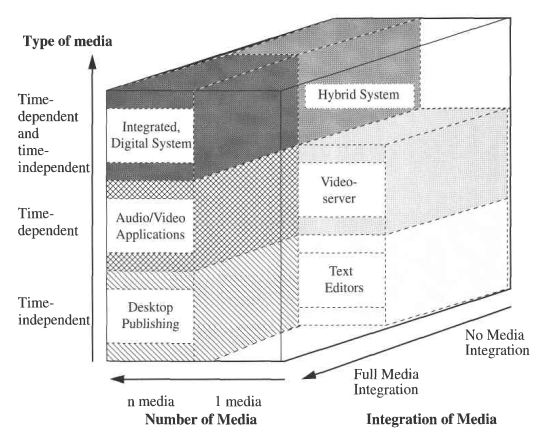
\includegraphics[width=0.8\textwidth]{media-classification}
	\caption{Classification of media use in multimedia systems.}
	\label{fig:media-classification}
\end{figure}
%--------------------------Figure end -------------------

Integral digital systems can support all types of media, and due to digital processing, may provide a high degree of media integration. Systems that handle time-dependent analog media objects and time-independent digital media objects are called \textit{hybrid systems}. The disadvantages of hybrid systems is that they are restricted with regard to the integration of time-dependent and time-independent media, for example, audio and video are stored on different devices than time-independent media objects.

The audio/video applications are time-dependent media objects. In addition, they often do not support the separate handling of audio and video media objects. They are supported by audio and video server.

Traditional desktop-publishing systems are examples of integrated processing of time-independent media objects supported by the text editors.

\subsubsection*{Basic Synchronization Issues}
The word synchronization refers to time. In a more general and wide sense, we use synchronization in multimedia systems as comprising:
\begin{itemize}
	\item \textit{content}
	\item \textit{spatial} and 
	\item \textit{temporal} relations between media objects
\end{itemize}


\paragraph*{Content Relations}
\begin{itemize}
	\item Content relations define a dependency of media objects from some data.
	\item Example: dependency between spreadsheet and graphics that represent data listed in spreadsheet. In this case, the same data are represented in two different ways.
	\item Another example is two graphics that are based on the same data but different interpretations of the data.
	\item In general, the implementation of content relations in multimedia systems is based on the use of common data structures or object interfaces that are used to present objects using different media.
\end{itemize}

\paragraph*{Spatial Relations}
\begin{itemize}
	\item The spatial relations that are usually known as \textit{layout relationship} define the space used for the presentation of a media object on an output device at a certain point of time in a multimedia presentation.
	\item In desktop-publishing applications, this is usually expressed using \textit{layout frames}. 
	\item A	layout frame is placed and a content is assigned to this frame. 
	\item The positioning of a layout frame in a document may be fixed to a position in a document, to a position on a page or it may be relative to the positioning of other frames.
\end{itemize}


\paragraph*{Temporal Relations}
\begin{multicols}{2}
	\begin{itemize}
		\item Temporal relations define the temporal (time) dependencies between media objects. 
		\item An example of temporal relations is the relation between a video and an audio object that are recorded during a concert. 
		\item If these objects are presented, the temporal relation during the presentations of the two media objects must correspond to the temporal relation at the recording moment.
	\end{itemize}
\end{multicols}


These time relations are synchronization in multimedia systems.


\subsubsection{Intra- and Inter-object Synchronization}

\paragraph*{Intra-object Synchronization}
\begin{multicols}{2}
	\begin{itemize}
		\item Intra-object synchronization refers to the time relation between various presentation units of one time-dependent media object. 
		\item An example is the time relation between the single frames of a video sequence. 
		\item For a video with a rate of $ 25 frames $ per second, each of the frames must be displayed for $ 40 ms $.
		\item Figure {\ref{fig:intra-object-sync}} shows this for a video sequence presenting a bouncing ball.
	\end{itemize}
\end{multicols}


%%%%%%%%%%%%%%%%%%%%%%%%%%%%%%%%%%%%%%%%%
%										%
%				FIGURE				   	%
%										%
%%%%%%%%%%%%%%%%%%%%%%%%%%%%%%%%%%%%%%%%%
\begin{figure}[ht!]
	\centering
	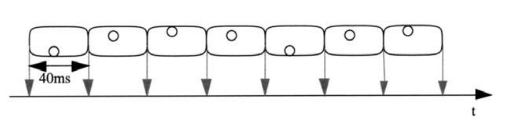
\includegraphics[width=0.8\textwidth]{intra-object-sync}
	\caption{Video sequence showing a bouncing ball.}\label{fig:intra-object-sync}
\end{figure}
%--------------------------Figure end -------------------


\begin{multicols}{2}
	\paragraph*{Inter-object Synchronization}
	\begin{itemize}
		\item Inter-object synchronization refers to the synchronization between media objects. 
		\item Figure {\ref{fig:inter-object-sync}} shows an example of the time	relations of a multimedia synchronization that starts with an audio/video sequence, followed by several pictures and an animation that is commented by an audio sequence.
	\end{itemize}
\end{multicols}



%%%%%%%%%%%%%%%%%%%%%%%%%%%%%%%%%%%%%%%%%
%										%
%				FIGURE				   	%
%										%
%%%%%%%%%%%%%%%%%%%%%%%%%%%%%%%%%%%%%%%%%
\begin{figure}[ht!]
	\centering
	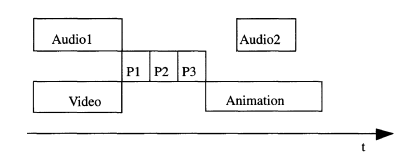
\includegraphics[width=0.8\textwidth]{inter-object-sync}
	\caption{Inter-object synchronization of images, one animation, and audiovisual	sequences.}\label{fig:inter-object-sync}
\end{figure}
%--------------------------Figure end -------------------



\subsection{Presentation Requirements}

\begin{multicols}{2}
	\begin{itemize}
		\item The correct transmission of multimedia data at the user interface requires synchronization. 
		\item It is impossible to state an objective measure for the synchronization from the view of the subjective human perception.
		\item As the human perception differs from one person to another, only heuristic criteria can be defined whether a presentation stream is correct.
	\end{itemize}
\end{multicols}
	
Requirements to the presentation include the accuracy with regard to the presentation of LDUs for intra-object synchronization, and the accuracy with regard to the parallelism of the presentation of media objects for inter-object synchronization. 

In intra-object synchronization, we should attempt to avoid jitter or variance in an two consecutive LDUs.

\subsubsection*{Live and Synthetic Synchronization}
The live and synthetic synchronization distinction refers to the type of the determination of temporal relations. In the case of live synchronization, the goal of the
synchronization is to exactly reproduce at a presentation the temporal relations as they existed during the capturing process. In the case of synthetic synchronization,
the temporal relations are artificially specified.

\subsubsection*{Live Synchronization}
\begin{multicols}{2}
	\begin{itemize}
		\item A typical application of live synchronization is conversational services. 
		\item In the scope of a source/sink scenario, at the source, volatile data streams (i.\ e.\ , data being captured from the environment) are created which are presented at the sink. 
		\item The common context of several streams on the source site must be preserved at the sink. 
		\item The source may be comprised of acoustic and optical sensors, as well as media conversion units. 
		\item The connection offers a data path between source and sink. 
		\item The sink presents the units to the user. 
		\item A source and sink may be located at different sites.
		\item The goal of synchronization in such a scenario is to reproduce at the sink the signals in the same way as they appeared at the source. 
		\item A possible manipulation by the sink is to adapt the presentation to the available resources.
		\item  This may be, for example, a change of resolution or a lower frame rate.
	\end{itemize}
\end{multicols}

\subsubsection*{Synthetic Synchronization}
The emphasis of synthetic synchronization is to support flexible synchronization relations between media. In synthetic synchronization, two phases can be distinguished:
\begin{multicols}{2}

	\begin{itemize}
		\item In the specification phase, temporal relations between the media objects are defined.
		\item In the presentation phase, a run-time system presents data in a synchronized mode.
	\end{itemize}
	
	
\end{multicols}

\subsection{Reference Model for Multimedia Synchronization}
A four-layer synchronization reference model is shown in Figure \ref{fig:sync-ref-model}.
\begin{multicols}{2}
	\begin{itemize}
		\item A reference model helps to understand the large number of requirements to multimedia synchronization. 
		\item Each layer implements synchronization mechanisms which are provided by an appropriate interface.
		\item These interfaces can be used to specify and/or enforce the temporal relationships.
		\item Each interface defines services, i.\ e.\ , offering the user a means to define his/her requirements. 
		\item Each interface can be used by an application directly, or by the next	higher layer to implement an interface.
		\item Higher layers offer higher programming and Quality of Service (QoS) abstractions.
	\end{itemize}
\end{multicols}


%%%%%%%%%%%%%%%%%%%%%%%%%%%%%%%%%%%%%%%%%
%										%
%				FIGURE				   	%
%										%
%%%%%%%%%%%%%%%%%%%%%%%%%%%%%%%%%%%%%%%%%
\begin{figure}[ht!]
	\centering
	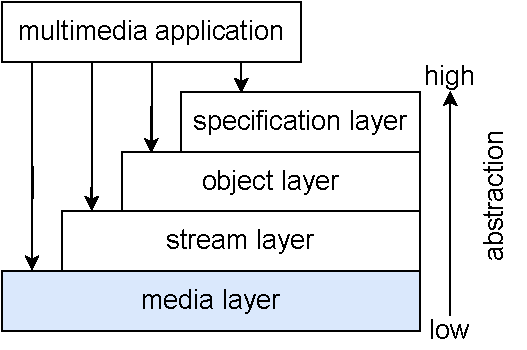
\includegraphics[width=0.7\textwidth]{sync-ref-model}
	\caption{A four-layer reference model.}\label{fig:sync-ref-model}
\end{figure}
%--------------------------Figure end -------------------


\subsubsection{Media Layer}
\begin{multicols}{2}
	\begin{itemize}
		\item On the media layer, an application handles one single continuous media stream as an LDU sequence. 
		\item The abstraction offered by this layer is a device-independent interface with operations like  \lstinline|read (device-handle, LOU)| and \lstinline|write (device-handle, LOU)|.
		\item To build a continuous media stream that uses the abstractions supplied by the	media layer, an application runs one process for each stream in the form shown in the
		following example:
	\end{itemize}
\end{multicols}

\begin{lstlisting}[frame=single]
window = open("Videodevice"); \\ Create a video output window
movie = open("File"); \\ Open the video file
while (not eof(movie)) { \\ Loop
	read (movie, &ldu); \\ Read LOU
	if (ldu.time == 20) \\ Start the presentation
		print("Subtitle 1"); \\ of the synchronized subtitles
	else if (ldu.time == 26)
		print ("Subtitle 2");
	write (window, ldu); \\ Present LOU
}
close(window);\\ Close window
close(movie); \\ Close file
\end{lstlisting}

\subsubsection{Stream Layer}
\begin{multicols}{2}
	\begin{itemize}
		\item The stream layer deals with continuous media streams and media stream groups. 
		\item A	group presents all streams in parallel by using mechanisms for inter-stream synchronization. 
		\item The abstraction supplied by the stream layer is called \textit{streams with time parameters}. 
		\item The quality of service relates to parameters for inter-stream synchronization	within a stream and inter-stream synchronization between the streams of the group.
		\item Continuous media in the stream layer are referred to as a data flow.
	\end{itemize}
\end{multicols}



\subsubsection{Object Layer}
\begin{multicols}{2}
\begin{itemize}
	\item The object layer deals with all kinds of media and hides the differences between discrete and continuous media from the user.
	\item The abstraction given by an application is that of a complete and synchronized presentation. 
	\item This layer accepts a synchronization specification as its input and is responsible for the correct scheduling (time plan) of the entire presentation.
	\item The object layer offers functions to calculate and execute complete presentation sequence schedules, including the presentation of non-continuous media objects.
	\item The object layer initiates preparatory actions required to achieve a correctly synchronized presentation.
	\item One example for the integration of this layer is the MHEG specification.
\end{itemize}
\end{multicols}

The objective of the MHEG standards is to encode multimedia and hypermedia information objects for presentation. Our example below uses a simple notation to
demonstrate the basics of this reference model.

\begin{lstlisting}[frame=single]
Composite { \\ Composite object
		start-up link \\ How to start the presentation
		viewer start-up 
		viewer-list \\ Virtual views on
		Viewerl: reference to Componentl \\ component objects
		Viewer2: reference to Component2
		Viewer3: reference to Component3
		Componentl \\ Component objects
			reference to content "movie.avs" \\ of the composite
		Component2
			reference to content "subtitle1"
		Component3
			reference to content "Subtitle2"
		Link1 \\ Temporal relations
			"when timestone status of Viewer1 becomes 20 then start Viewer2"
		Link2 
			"when timestone status of Viewer1 becomes 26 then start Viewer3"		
}
\end{lstlisting}

One possible implementation of the object layer is the MHEG runtime system called \textit{MHEG Engine}. This engine evaluates the status of the objects and executes operations
(actions), e.\ g.\ , to prepare, start, stop, or destroy objects.

\subsubsection{Specification Layer}
\begin{multicols}{2}
\begin{itemize}
	\item The specification layer is an ``open'' layer. 
	\item It does not provide for an explicit interface.
	\item This layer includes applications and tools that can be used to generate synchronization specifications.
	\item Such tools include editors for synchronization and multimedia document and authoring systems, and tools used to convert specifications into an object-layer format.
	\item The specification layer is also responsible for mapping QoS requirements of the user level to the qualities offered at the object layer interface.
\end{itemize}
\end{multicols}

The methods used to specify synchronization can be grouped into the following main categories:

\begin{itemize}
	\item \textit{Interval-based specifications}, which allow the specification of temporal relationships between the time intervals of the presentation of media objects.
	\item \textit{Axis-based specifications}, which set the presentation results in relation to the axes, which are used jointly by the presentation objects.
	\item \textit{Control-flow-based specifications}, where the presentation flow is synchronized at specific synchronization points.
	\item \textit{Events-based specifications}, where the events of the presentation of media are stated to trigger presentation actions.
\end{itemize}	

%%%%%%%%%%%%%%%%%%%%%%%%%%%

% 			TABLE	 	 %

%%%%%%%%%%%%%%%%%%%%%%%%%%%
\begin{landscape}
	\begin{longtable}[c]{@{}p{3cm}p{8cm}p{5cm}@{}}
		\caption{Overview on the layers of the synchronization reference model.}
		\label{tab:sync-reference-model-overview}\\
		\toprule
		\textbf{Layer} & \textbf{Interface Abstraction}                     & \textbf{Tasks}                                                       \\* \midrule
		\endfirsthead
		%
		\multicolumn{3}{c}%
		{{\bfseries Table \thetable\ continued from previous page}} \\
		\toprule
		\textbf{Layer} & \textbf{Interface Abstraction}                     & \textbf{Tasks}                                                       \\* \midrule
		\endhead
		%
		\bottomrule
		\endfoot
		%
		\endlastfoot
		%
Specification &	{The tools performing the tasks of this layer have interfaces; the layer itself has no upper interface\par} & {Editing\par Formatting\par Mapping user-oriented QoS to the Qos abstraction at the object layer\par}\\
	
Object  &{Synchronization specification\par Objects hiding the types of integrated media\par Media-oriented QoS (with regard to the acceptable skew and jitter)\par}  & {Plan and coordinate presentation schedules\par  Initiate the presentation of continuous media objects in the stream layer\par Initiate the presentation of discrete media objects \par Initiate presentation preparation actions }\\

Stream & {Arrange streams and stream groups\par Supply guarantees for intra-stream synchronization\par Supply guarantees for interstream synchronization\par}   & Reserve resources and schedule LDU processing\\
Media  & {Provide device-independent access to LDUs\par Supply guarantees for single LDU processing} & File and device access \\* \bottomrule
	\end{longtable}
\end{landscape}

\subsection{Synchronization Specification}
\begin{multicols}{2}
	\begin{itemize}
		\item The synchronization specification of a multimedia object describes all \textit{temporal dependencies} of the embedded objects. 
		\item It is generated by means of tools offered in the specification layer and used at the interface to the object layer. 
		\item The synchronization defines the entire presentation, so that it represents a central task in multimedia systems.
		\item The following list describes and evaluates the requirements to the synchronization specification and specification methods.
	\end{itemize}
\end{multicols}


A synchronization specification should consist of the following components:

\begin{multicols}{2}
	\begin{itemize}
		\item Intra-object specification for the media objects embedded in the presentation.
		\item Description of the QoS parameters for intra-object synchronization.
		\item Specification of the inter-object synchronization for media objects embedded in the presentation.
		\item Description of the QoS parameters for inter-object synchronization.
	\end{itemize}
\end{multicols}


The synchronization specification is part of the description of a multimedia object. In addition, it can describe the form to be used to represent a media object. For example, a piece of text could be written in the form of characters on the screen or generated as audio sequence. A specification can allow either of these two options or a choice of presentation forms at runtime.

For live synchronization, the temporal relationships are defined implicitly during the recording phase. The QoS requirements of each of the media involved are determined at the beginning of the recording phase.

If synthetic synchronization is applied, then the specification has to be explicitly created. 

\subsection*{Specification Methods for Multimedia Synchronization}
Complex specifications for multiple object synchronizations, including user interaction, require highly developed specification methods. The following requirements should be met by such a specification method:

\begin{multicols}{2}
	\begin{itemize}
		\item Should support object consistency and maintenance of synchronization specifications.
		\item Should supply an abstraction of the contents of each media object.	
		\item Should allow easy description of all types of synchronization relationships.
		\item Should support the integration of continuous and discrete media objects.
		\item Should support the definition of QoS requirements.
		\item In addition, the method should support hierarchical synchronization levels to facilitate the processing of large and complex synchronization scenarios.
	\end{itemize}
\end{multicols}

Following are the specification methods based on the above criteria.

\subsubsection{Interval-based Specification}
An interval-based synchronization specification considers the duration of the presentation of an object as an interval. Two time intervals can be synchronized in 13 different
types, where some of these types can be inverted. 

Figure \ref{fig:interval-based-spec} shows section of seven non-inverted rates. A simple method for synchronization specification of two media objects is able to use these seven types.


\begin{figure}[ht!]
	\centering
	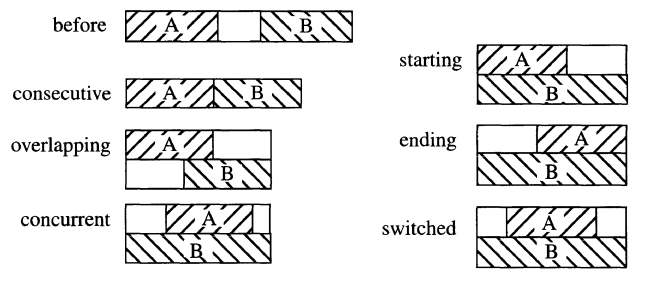
\includegraphics[width=0.7\textwidth]{interval-based-spec}
	\caption{Types of temporal relationships between two objects.}
	\label{fig:interval-based-spec}
\end{figure}

\paragraph*{Benefits}
\begin{multicols}{2}
	\begin{itemize}
		\item Logical objects can be maintained.
		\item Good abstraction of media contents.
		\item Easy integration of discrete objects.
		\item Easy integration of interactive objects.
		\item Supports the specification of unknown temporal relations.
	\end{itemize}
\end{multicols}


\paragraph*{Drawbacks}
\begin{multicols}{2}
\begin{itemize}
	\item The specification is complex.
	\item Allows direct specification of temporal relationships between media objects, but not for subunits of media objects.
	\item Resolution of unknown relations at runtime can cause inconsistencies.
\end{itemize}
\end{multicols}


\subsubsection{Axis-based Synchronization}
Axis-based synchronization means that presentation events, such as start and end of a presentation, are mapped to axes, which are common to all objects of a presentation.

\paragraph*{Synchronization Based on a Global Timer}
\begin{multicols}{2}
	\begin{itemize}
		\item To implement a synchronization based on a global timer, all individual media objects are bound to an axis, representing an abstraction of the real world. 
		\item This method describes the synchronization by linking all objects. 
		\item They are mapped independently on a time axis. 
		\item This means that the removal of one object does not influence the synchronization of the other objects.
	\end{itemize}
\end{multicols}

\subparagraph*{Benefits}
\begin{multicols}{2}
	\begin{itemize}
		\item Easy to understand.
		\item Supports easy implementation of hierarchies.
		\item Easy integration of discrete objects.
		\item Easy handling of objects thanks to mutual independence.
		\item Good abstraction of media contents.
	\end{itemize}
\end{multicols}



\subparagraph*{Drawbacks}

\begin{multicols}{2}
	\begin{itemize}
		\item Objects with unknown duration cannot be integrated; expansions to this model are required.
		\item The QoS skew has to be defined indirectly by a common time axis or additional QoS specification.
	\end{itemize}
\end{multicols}

\paragraph*{Synchronization Based on Virtual Axes}
We can use this specification method to specify coordinated systems with user-defined measurement units.

\subsubsection{Control-flow-based Specification}
Specifications based on the control flow synchronize the flow of coinciding presentation processes at predefined points within the presentation

\paragraph*{Basic Hierarchical Specification}
Hierarchical synchronization descriptions are based on two main synchronization operations: the serial synchronization and the parallel synchronization.


\paragraph*{Reference Points Specification}
In synchronization over reference points, continuous single media objects are handled as sequences of closed LDUs.

\paragraph*{Time-specific Petri Networks}
Another type of specification is based on Petri networks, which expands the time specifications at various points.

\subsubsection{Events-based Synchronization}
In an events-based synchronization, presentation actions are initiated by synchronization events. Typical presentation actions are:
\begin{itemize}
\item Start a presentation. 
\item Stop a presentation. 
\item Prepare a presentation.
\end{itemize}


\newpage\thispagestyle{empty}
